\documentclass[12pt]{article}
%%%% Load Packages %%%%
\usepackage[utf8]{inputenc}
\usepackage[english]{babel}
\usepackage{indentfirst}
\usepackage{color}
% \usepackage{url}
\usepackage{hyperref}
\usepackage[citestyle=authoryear, bibstyle=authoryear, sorting=nyt]{biblatex}
\usepackage{caption}
% \usepackage{etoolbox}
\usepackage{fancyhdr}
\usepackage{geometry} %[margin=1in]
%\usepackage[absolute]{textpos}
\geometry{
	top=1in, % Top margin
	bottom=1in, % Bottom margin
	left=1in, % Left margin
	right=1in, % Right margin
%	showframe, % Uncomment to show how the type block is set on the page
}
\usepackage{pdflscape}
\usepackage{graphicx}
\usepackage{parskip}
\usepackage{setspace}
\usepackage{titlesec}
\usepackage{titletoc}
\usepackage{booktabs}
\usepackage{multirow}
%\usepackage{endnotes} % Use end notes instead of footnotes
%\let\footnote=\endnote % Use end notes instead of footnotes

% Adjust marginparwidth before loading todonotes/changes
\setlength{\marginparwidth}{2cm}
\usepackage{changes} % Use [final] to accept all changes; remove [final] to track changes
% Define author for suggestions
\definechangesauthor[name={Matt Carson}, color=red]{MC}

\usepackage[autostyle, english = american]{csquotes}
\MakeOuterQuote{"}
\usepackage[acronym, nogroupskip]{glossaries}
\makeglossaries

%\titleformat{\section}{\fontsize{12}{14}\bfseries\centering}{\thesection}{0.5em}{}

%%%% Include acronyms file %%%%
%%%% List of Acronyms and abbreviations %%%%

\newacronym{afl}{AFL}{American Federation of Labor}
\newacronym{aflcio}{AFL-CIO}{American Federation of Labor-Congress of Industrial Organizations}
\newacronym{anga}{ANGA}{America's Natural Gas Alliance}
\newacronym{btc}{BTC}{Building Trades Council}
\newacronym{cba}{CBA}{Collective Bargaining Agreement}
\newacronym{cio}{CIO}{Congress of Industrial Organizations}
\newacronym{csb}{CSB}{U.S. Chemical Safety and Hazard Investigation Board}
\newacronym[
    description={Community Workforce Agreement (also called Project Labor Agreement [PLA])}
]{cwa}{CWA}{Community Workforce Agreement}
\newacronym{dapl}{DAPL}{Dakota Access Pipeline}
\newacronym{efca}{EFCA}{Employee Free Choice Act}
\newacronym{iam}{IAM}{International Association of Machinists and Aerospace Workers}
\newacronym{ibew}{IBEW}{International Brotherhood of Electrical Workers}
\newacronym{ilgwu}{ILGWU}{International Ladies Garment Workers Union}
\newacronym{ilwu}{ILWU}{International Longshore and Warehouse Union}
\newacronym{iupat}{IUPAT}{International Union of Painters and Allied Trades}
\newacronym{iww}{IWW}{Industrial Workers of the World}
\newacronym{jatc}{JATC}{Joint Apprenticeship Training Committee}
\newacronym{lcca}{LCCA}{Labor Coalition for Community Action}
\newacronym{lcsp}{LCSP}{Labor Campaign for Single Payer}
\newacronym{liuna}{LIUNA}{Laborers' International Union of North America}
\newacronym{lmrda}{LMRDA}{Landrum-Griffin Labor-Management Reporting and Disclosure Act}
\newacronym{nabtu}{NABTU}{North America's Building Trades Unions}
\newacronym{nepa}{NEPA}{National Environmental Policy Act}
\newacronym{nlra}{NLRA}{National Labor Relations Act}
\newacronym{nlrb}{NLRB}{National Labor Relations Board}
\newacronym{ocaw}{OCAW}{Oil, Chemical and Atomic Workers Union}
\newacronym{opcima}{OPCIMA}{Operative Plasterers' and Cement Masons' International Association}
\newacronym{oshact}{OSH Act}{Occupational Safety and Health Act}
\newacronym{owiu}{OWIU}{Oil Workers International Union}
\newacronym{pace}{PACE}{Paper, Allied-Industrial, Chemical, and Energy Workers International Union}
\newacronym[
    description={Project Labor Agreement (also called Community Workforce Agreement [CWA])}
]{pla}{PLA}{Project Labor Agreement}
\newacronym{proact}{PRO Act}{Protecting the Right to Organize Act}
\newacronym{rwdsu}{RWDSU}{Retail, Wholesale, and Department Store Union}
\newacronym{seiu}{SEIU}{Service Employees International Union}
\newacronym[
	description={United Association of Journeymen and Apprentices of the Plumbing and Pipe Fitting Industry}]
	{ua}{UA}{United Association of Plumbers and Pipefitters}
\newacronym{uaw}{UAW}{United Auto Workers}
\newacronym{ufcw}{UFCW}{United Food and Commercial Workers}
\newacronym{ugccwa}{UGCCWA}{United Gas, Coke, and Chemical Workers of America}
\newacronym{umwa}{UMWA}{United Mine Workers of America}
\newacronym{upiu}{UPIU}{United Paperworkers' International Union}
\newacronym[
	description={United Steel, Paper and Forestry, Rubber, Manufacturing, Energy, Allied Industrial and Service Workers International Union}
]{usw}{USW}{United Steelworkers}

%%%% Head height %%%%
\setlength{\headheight}{15pt}

%%%% Line spacing %%%%
\setstretch{2}

%%%% Paragraph spacing %%%%
\setlength{\parskip}{0pt}

%%%% Define indentation length %%%%
\newlength{\myindent}
\setlength{\myindent}{0.5in}

%%%% Set the hanging indent %%%%
\setlength{\bibhang}{\myindent}

\AtEveryBibitem{
	\clearfield{issn}
	\ifentrytype{book}{\clearfield{isbn}}{}
    \clearfield{urlyear}
    \clearfield{urlmonth}
    \clearfield{urlday}
}

%%%% Redefine the citation command to use a colon instead of a comma and pp. %%%%
\DeclareFieldFormat{postnote}{#1}
\DeclareFieldFormat{multipostnote}{#1}

% Redefine the URL format to not use \texttt style
%\DeclareFieldFormat{url}{\href{#1}{#1}} % This will format the URL in the regular text font

% Optionally, redefine the DOI and eprint formats similarly if you use them
%\DeclareFieldFormat{doi}{\href{https://doi.org/#1}{#1}}
%\DeclareFieldFormat{eprint}{\href{https://arxiv.org/abs/#1}{#1}}

%%%% Use colon (ASA Style) in-text citations (author year: page) %%%%
\renewcommand*{\postnotedelim}{\addcolon}

%%%% Set global text alignment to ragged-right %%%%
%\raggedright

%%%% Paragraph indentation %%%%
\setlength{\parindent}{\myindent}

%%%% Font %%%%
% \setmainfont{Times New Roman}

%%%% Define variables for reused text or dimensions %%%%
% Full title
\newcommand{\fullTitle}{Construction Union Agreements:\par{}Union Organizing in Historical-Comparative Perspective}
% Short title
\newcommand{\shortTitle}{CONSTRUCTION UNION AGREEMENTS}

% Standardize image width
\newcommand{\imageWidth}{0.8\textwidth}

%%%% Page style %%%%
\pagestyle{fancy}
\fancyhf{} % clear all header and footer fields
%\fancyhead[R]{\thepage} % page number on the right side
\fancyhead[R]{\hyperlink{toc}{\thepage}} % page number on the right side, linked to the TOC
\fancyhead[L]{\small \shortTitle}
\renewcommand{\headrulewidth}{1pt} % header rule

% Customize abstract page
\renewenvironment{abstract}
  {\par\noindent\centering\textbf{\fullTitle}\par}
  {\noindent\raggedright}
%  {\par}

% Redefine the quote environment
\renewenvironment{quote}
  {\list{}{\leftmargin=\parindent\rightmargin=0pt}%
   \item\relax}
  {\endlist}
  
% Redefine the quote environment to make it single-spaced 
% and remove vertical space before and add one at the end
\AtBeginEnvironment{quote}{\singlespacing\setlength{\topsep}{0pt}\setlength{\partopsep}{0pt}}
\AtEndEnvironment{quote}{\vspace{0.5\baselineskip}}

% Custom command \acrparen to place acronyms in parentheses
% \acrparen
\newcommand{\acrparen}[1]{(\acrshort{#1})}

% Custom command to reference section number and name
% \fullref
\addto\extrasenglish{\def\sectionautorefname{Section}}
\addto\extrasenglish{\def\subsectionautorefname{Section}}
\addto\extrasenglish{\def\subsubsectionautorefname{Section}}
\newcommand{\fullref}[1]{\autoref{#1}: ``\nameref{#1}"}

% Command to use \textcite in the possessive form
\newcommand{\poscite}[1]{\citeauthor{#1}'s (\citeyear{#1})}
%	%%%%%%%%%%%%%%%
%			Document Begins         %
%			Preliminary Pages 		  %
%	%%%%%%%%%%%%%%%
\addbibresource{1_SOC_Honors.bib}
%%%% Title Page %%%%
\begin{document}
\setstretch{1.25} % Set line spacing
\begin{titlepage}
  \thispagestyle{fancy}
  \pagenumbering{gobble} % Turn off page numbering for the title page
  \fancyhead[L]{Running Head = \shortTitle}
  \renewcommand{\headrulewidth}{0pt} % header rule
  \centering
  \vspace*{2in}
  \fullTitle\par
  \vspace{1.2in}
  {Matthew A. Carson\par}
  \vspace{12pt}
  Department of Sociology\par
  University of California, Los Angeles\par
  \vspace{0.5in}
  {\today\par}
%  \vfill
%  \wordcount
\end{titlepage}

% Blank page so that the abstract does not begin on the back of the cover page.
% Blank page
\thispagestyle{empty} % Remove header and footer

\vspace*{\fill}
\hspace*{\fill}
\begin{center}
    \noindent{}\textit{This page intentionally left blank}
\end{center}
\hspace*{\fill}
\vspace*{\fill}

\clearpage

% Set page numbering to Roman for preliminary pages
\pagenumbering{roman}
\setstretch{2}
%\titlespacing*{\abstract}{0pt}{0pt}{0pt}

% Add abstract page
\begin{abstract}
US Building Trade unions organize their workers differently. Most labor unions compel employers to negotiate, but the Building Trades engage in voluntary negotiations, relying on workers' skill levels rather than strike leverage. This approach correlates with their frequent political deviations from the broader US labor movement, particularly in opposing progressive environmental policies, aligning more closely with the petrochemical industry on environmental issues, and not supporting single-payer healthcare. One view is that unions pursue their members’ interests narrowly, sacrificing broader working-class interests if they feel it is necessary to secure work for their members, and some suggest that the conservative stance of the Building Trades stems from their craft union tradition, in which workers are organized by craft and skill instead of by industry. However, using historical-comparative methods, I show that these arguments do not hold. Petrochemical unions have supported progressive policies, and other craft-based unions have endorsed single-payer healthcare. However, unlike the Building Trades, those unions have never used voluntary agreements. Consequently, they have experienced more conflicts with employers. These findings challenge traditional views and suggest that the Building Trades' conservative negotiation strategies significantly shape their political and policy positions, reinforcing an employer-union dynamic that limits challenging management.
\end{abstract}

\clearpage

% Add table of contents (TOC)
\setstretch{1.25}
\hypertarget{toc}{}
\tableofcontents
%\clearpage

% List of Figures
\listoffigures

% List of tables
\listoftables

%\clearpage
% List of acronyms
%\addcontentsline{toc}{section}{Acronyms}
%\setglossarystyle{listgroup}
\printglossary[type=\acronymtype,title=Acronyms]

\clearpage

%	%%%%%%%%%%%%%%%%%%%	%
% Define custom section headings			%
%	%%%%%%%%%%%%%%%%%%%	%
%%%% Parts %%%%
\titleformat{\part}[block]
	{\normalfont\Large\bfseries}
	{\thepart.}
	{6pt}
	{\Large\MakeUppercase}

%%%% Sections %%%%%
\titleformat{\section}[block]
	{\normalfont\fontsize{12}{14}\selectfont\bfseries}
	{\thesection.}
	{0.25em}
	{}

%%%% Subsections %%%%
\titleformat{\subsection}[block]
	{\itshape\bfseries}
	{} % \thesubsection.
	{0pt} % 0.25em
	{}

%%%% Subsubsections %%%%
\titleformat{\subsubsection}[runin]
	{\normalfont\itshape\bfseries}
	{\hspace{\myindent}} % \thesubsubsection.
	{0pt} % 0.25em
	{}[.]%{\hspace{0em}}%[\hspace{2pt}]

%%%% Paragraphs %%%%
\titleformat{\paragraph}[runin]
	{\normalfont\itshape\bfseries} % Normal font, italic, bold
	{} % \hspace{\myindent}\theparagraph. % Label (you can add numbering here if needed)
	{0.25em} % Separation between the label and the title
	{} % Additional formatting
	[.]

% Adjust spacing before and after sectioning commands
\titlespacing*{\part}{0pt}{0pt}{10pt}
\titlespacing*{\section}{0pt}{0pt}{0pt} % \baselineskip
\titlespacing*{\subsection}{0pt}{0pt}{0pt}
\titlespacing*{\subsubsection}{0pt}{0pt}{0.5em}
\titlespacing*{\paragraph}
  {\myindent} % Left margin (you can set this to \parindent to align with paragraph indentation)
  {0pt} % Space before the paragraph title
  {0.5em} % Space after the paragraph title

% \titlecontents{subsubsection}
  % [5em]                       % 1. Indentation
  % {}                          % 2. Above code
  % {}                          % 3. Numbered entry format
  % {}                          % 4. Formatting of numbered entry
  % {\hspace{0.25em}\titlerule*[0.75em]{.}\contentspage}       % 5. Page number format
  % []                          % 6. Below code


%%%%%%%%%%%%%%%%%%%%%%%
%%					Main document starts			  %%
%%%%%%%%%%%%%%%%%%%%%%%
% Set to double-spacing
\setstretch{2}

% Preface
\addcontentsline{toc}{section}{Preface}
\section*{Preface}\label{preface}

My interest in this topic began sometime in the late aughts or early 2010s. This was around the time that there was much talk about the \acrfull{efca}, which, like the \acrfull{proact} legislation of 2021, would allow unions to use cards that workers sign to indicate that they want a union in their workplace (often condensed into the term "union representation"). There was (and is) a tremendous amount of effort that most employers will expend to keep their workplaces from unionizing. At the time, Wal-Mart and other grocery stores were big targets for unionization by the \acrfull{ufcw}, as was the service sector in general. Amid fierce opposition from employers, organizing campaigns were largely unsuccessful. 

\acrshort{efca} was seen as a way to "level the playing field," as it were. Current labor law allows employers to insist on a secret ballot election whenever a union claims that it has support from a majority of the workers. The employer \emph{could} accept that the union has majority support and begin bargaining with the union as soon as the union presents evidence of the same (e.g., cards signed by the majority of the workers), but this rarely happens because by insisting on conducting an election, the employer has time to conduct an anti-union campaign, usually by professional union busting firms. Supporters of \acrshort{efca} contended that allowing the employer to require a secret ballot election \emph{after} the majority of workers had already signed cards shifted conditions heavily in favor of the employer, and such a process was superfluous because majority status had already been demonstrated.

At the time, I was a newly admitted plumbing apprentice. The story of union organizers facing fierce anti-union opposition did not square with my experience in the \acrfull{ua}. Union officials and members alike were more apt to describe the union-employer relationship as mutually beneficial, not conflictual, or the employers and union members as a team. "They need us, and we need them" was a common refrain. While in a mundane sense, it is true enough that employers need workers to build their projects and workers need employment so that they can eat, that certainly is not limited to construction. Yet, the way that construction unions talked about employer-union relations was strikingly different from the way that the rest of organized labor was talking. Moreover, construction unions were generally silent on the issue of having the organizing conditions tilted in favor of management. But why?

That is when I discovered that construction unions have an entirely different contract type that does not require them to organize like other unions do. Instead of conducting workplace organizing the way that the rest of the labor movement does, construction unions can \emph{voluntarily} enter into agreements with employers, meaning that rather than fiercely opposing unionization like most employers do, construction employers \emph{voluntarily} went to the union to hire a unionized workforce. But why would they do that while nearly every non-construction employer was fiercely opposed to unions? I was puzzled. This led me to begin thinking about power dynamics in construction unions vis-\`a-vis the rest of organized labor. This project is the product of a number of years of thinking about those dynamics.

I have had the good fortune of being assisted by Dr. Zsuzsa Berend and Zep Kalb. What started vaguely as a project studying power dynamics and class collaboration in construction unions, where I was really only thinking of fleshing out the internal logic of class collaboration in US construction unions, evolved into a historical-comparative project. I deeply appreciate their patience with me as I evolved in my thinking on how to best approach the question. Moreover, because the topic is familiar to me, both through personal experience and thinking about it for a number of years, it was easy to forget that certain ideas and concepts, especially those particular to this odd business of US construction unionism, were not immediately clear to others. So, their feedback throughout the project helped tremendously.

\clearpage
% Blank page
\thispagestyle{empty} % Remove header and footer

\vspace*{\fill}
\hspace*{\fill}
\begin{center}
    \noindent{}\textit{This page intentionally left blank}
\end{center}
\hspace*{\fill}
\vspace*{\fill}

\clearpage
%%%%%%%%%%%%%%%%%%%%%%%
%%					INTRODUCTION					  %%
%%%%%%%%%%%%%%%%%%%%%%%
% Set page numbering to Arabic for main content
\pagenumbering{arabic}

%\phantomsection
%\addcontentsline{toc}{section}{Introduction}
\section{Introduction}\label{introduction}

Do the ways that unions organize affect their political stances? US construction unions have a distinct approach to organizing their workers vis-à-vis other labor unions. While most labor unions typically compel employers to negotiate through secret ballot elections or work stoppages, the Building Trades take a different route by engaging in voluntary negotiations.\footnote{See \autoref{modes_of_bargaining} for a discussion of the history of secret ballot elections and how the Building Trades negotiates.} Their strategy hinges more on the skill levels of their workers than the leverage of strikes or official \acrfull{nlrb} elections, which use the state to compel the employer to negotiate. At the same time, the Building Trades are often outliers in the US labor movement. They frequently oppose progressive environmental policies and thus align more closely with their employers in the petrochemical industry than with other labor or environmental organizations on environmental issues. Additionally, they are not supportive of single-payer healthcare or other social wage policies.\footnote{To be sure, not all non-Building Trades unions endorse or support single-payer healthcare, but \emph{no} Building Trades unions do at the national level.} Why have the Building Trades taken these positions?

One potential explanation is that unions with many workers in the petrochemical industry will align with the employer on environmental policy if they believe environmental policies might be "job killers." That is, the Building Trades' opposition to an environmental policy meant to attenuate global warming might simply be a function of the union's interest in keeping their members working. The building trades have many members working on projects in the petrochemical industry, and from this perspective, this is what one would expect from workers and their unions in that industry. After all, why would they support something that might cause unemployment?

Still, others argue that the conservative stance of the Building Trades originates from their tradition of craft unionism, where workers are organized based on craft and skill rather than industry (\cite{roginComment1974, perlmanHistoryTradeUnionism1922, issermanGodBlessOur1976, fonerHistoryLaborMovement1996}). Craft unions were some of the earliest labor organizations in the US. Their focus on organizing narrowly based on craft distinctions (e.g., plumber) rather than by industry (e.g., construction worker) often corresponded with nativist and racist policies and more conservative positions (e.g., anti-communism and redbaiting), while industrial unions more often opposed racism and were more militant (\cite{fonerHistoryLaborMovement1994}). In short, craft unions have tended to look out for "their own" more than workers more broadly.\footnote{There are dissenting views concerning how politically conservative the \acrshort{afl} craft unions were. See \citeauthor{cobblePureSimpleRadicalism2013} (\citeyear{cobblePureSimpleRadicalism2013}) for a dissenting scholarly article, and \citeauthor{parkerAreIndustrialUnions2008} (\citeyear{parkerAreIndustrialUnions2008}) for a union activist's perspective on the nature of craft and industrial unionism.} The Building Trades unions continue to operate as craft unions today.\footnote{One can find a union for almost every construction craft---electricians, plumbers, bricklayers, and so on---but good luck finding a union called the "Construction Workers Union."} From this perspective, the Building Trades' conservativism stems from their narrow, craft-based unionism.

However, these views offer an incomplete picture. For instance, some unions with many members working in the petrochemical industry, such as the United Steelworkers (\acrshort{usw}), have backed progressive policies, including environmental policies, and other craft-based unions, such as the \acrfull{iam}, have endorsed single-payer healthcare despite organizing along craft lines instead of industry. The key distinction between these unions and their disparate political stances lies in the Building Trades' use of voluntary agreements, which minimizes conflicts with employers and constrains their ability to challenge management.

\subsection*{Overview}\label{overview}

After reviewing the literature (\autoref{lit_review}) and introducing the methods (\autoref{methods}), \fullref{craft_vs_industrial} introduces the older craft union logic that the first major US labor federation was guided by and that many unions still adhere to today and contrasts it with the industrial unionism that emerged in response to growing factory production and the perceived inadequacies of craft unionism. \fullref{modes_of_bargaining} contrasts the two types of union bargaining and contracts, and \fullref{outlier} situates the building trades as an outlier in the broader context of the US labor movement by discussing the \acrfull{dapl}. In \fullref{union_shareholders}, Sean McGarvey reveals in an interview that the \acrfull{nabtu} union philosophy conceives of union members as "shareholders" whose interests are best served by helping their employer be successful and never striking. \fullref{interunion_cases} introduces the inter-union\footnote{Between building trades and non-building trades unions} comparative cases and their historical background. 

In addition to several inter-union comparisons, I also conducted several interviews with building trades organizers for intra-building trades comparisons. A minority of building trades unions organized workers using the non-construction method. I suspected that these unions might have more progressive politics because they had decided to use a more conflictual or coercive organizing approach. I analyze these interviews in \fullref{intracases} and find that, in general, the construction unions that organize using the non-construction method do not embrace more progressive politics.

\section{Literature Review}\label{lit_review}

Nearly every project conducted since the 1980s that studied construction unions begins with an acknowledgment that construction unions have been underresearched. Alas, not much has changed in the past forty years. From historians and economists, the national-level histories are sparse and dated \parencite{segalRiseUnitedAssociation1970, christieEmpireWoodHistory1956}. These provide valuable data on the early origins of the unions but, of course, do not tell one much about the present state of affairs. Like the national-level analyses, local and regional-level histories have been sparse, and many were completed in the 1990s or earlier \parencite{schneirovPrideSolidarityHistory1993, kazinBaronsLaborSan1989}. These works have also tended to be more idiographic, so while they offer extremely valuable insight, they have generally not been in conversation with one another in an attempt to build a more general theory of construction union organizing and leverage.

%\textcite{silverConstructionWorkAlienation1986} studied the 

\subsection{Race and Gender}

Other authors explore the dynamics of race and gender in the building trades, highlighting the persistent hard-hat culture where masculinity is defined by physical prowess and bravery. They contend that this machismo is not only a reaction to the dangers of the job but also a way for workers to assert their identity in the face of unsafe working conditions and fear of reprisals \parencite{moccioContradictingMalePower1992, paapWorkingConstructionWhy2006}. Tradesmen often deal with unsafe environments by accepting monetary compensation instead of confronting contractors, thereby reinforcing a self-consciously macho image to cope with the risks without losing face \parencite{moccioContradictingMalePower1992}. \textcite{paapWorkingConstructionWhy2006} delves further into the complex interplay of gender, race, and class within the construction industry, arguing that the performative expectations of masculinity, which she terms "pigness," compel white male workers to engage in behaviors that ultimately weaken their position within the employment market. These behaviors include working harder and more dangerously to prove their worth to their employers, thereby commodifying their bodies in a way that erodes their negotiating power and long-term ability to work. \textcite{paapWorkingConstructionWhy2006} highlights that these practices not only harm individual workers but also undermine the union movement and the working class as a whole.

The image of the building trades as an Archie Bunkeresque "good old boys" club that excludes women and people of color is pervasive. However, it only offers an incomplete picture. For example, unions such as the \acrfull{liuna} are heavily Latino, but they are hardly bastions of egalitarianism. Indeed, sociologist David \textcite{fitzgeraldTransnationalismMexicanHometown2004}, in his study of transnationalism, found that the Southern California laborers local union in his study had a patronage network that excluded many first and second-generation Mexican-American laborers from the more desirable jobs in the union. Instead, \emph{Guadalupanos} were given priority based on their connections to hometown networks in Mexico. This hardly squares with the good old boys picture that one gets from \textcite{paapWorkingConstructionWhy2006}.

The emphasis on worker "machoness" also sidesteps the issue of employer responsibility. In a discussion of the "Big Blue" crane collapse that killed three workers at the then-under-construction Milwaukee Brewers' stadium, \textcite{paapWorkingConstructionWhy2006} contends that the workers' masculinities put them in harm's way. \citeauthor{paapWorkingConstructionWhy2006} contends that the men felt tremendous pressure to look tough and thus decided to conduct crane operations in high winds despite the danger and violation of \acrfull{oshact} regulations. \citeauthor{paapWorkingConstructionWhy2006}, like the employer, contends that the men voluntarily put themselves in harm's way instead of refusing to complete the unsafe task. However, this sidesteps the issue of holding the employer accountable and significantly overlooks the power differential between the employer and workers.

Workers, especially in construction work, have contingent, temporary employment and tend to have little protection from arbitrary firings. Though \emph{de jure} protection exists from retaliatory firings for refusing to do unsafe work both by law and typically also by \acrfull{cba} language, the contingent, temporary nature of the work makes it difficult to prove retaliation. Often employers will retaliate with "reduction in force" (i.e., a claim that there is a lack of work to keep someone employed) as a pretext. And since typically all that is needed to successfully fight a retailiation case is evidence that the employer had a legitimate business reason to lay someone off, the claim that the job was "winding down" will usually suffice absent some other evidence that shows that the employer harbored animus over a refusal to work in unsafe conditions.

Moreover, a reputation as a union "troublemaker" could likely follow one throughout their time within the union even after a retaliatory "layoff." This, coupled with the fact that a layoff can often mean months of unemployment, makes refusing unsafe work much more difficult and fraught with worries about financial stability---paying rent, purchasing food, etc.---than \citeauthor{paapWorkingConstructionWhy2006} portrays it. So while it is tempting to simply say that the workers should have turned down the unsafe task and rejected whatever masculine inclinations they have, the reality is much more complicated.

To be sure, there is significanty occupational segregation in the building trades, mostly between unions classified as "basic crafts," laborers, roofers, cement finishers, etc. and the "skilled crafts," plumbers, pipe fitters, electricians, elevator constructors, etc. Blacks and especially Latinos are disporportionately employed in the "basic crafts," which usually have lower pay and less generous benefits, while the "skilled crafts" are disproportionately white.\footnote{Statistics by craft are difficult to find. Much of this is based on my personal observations during 10 years as a union construction worker. While I am fully aware that my experience might not be representative, it is well-documented that the "basic crafts" are comprised heavily of Latino, immigrant workers (See, for example, \textcite{erlichStandingCrossroadsBuilding2005, grabelskyConstructionDeConstructionRoad2007}).} Across all unions, women are substantially underrepresented at only four percent of the unionized sector despite being 14 percent of the construction workforce \parencite{u.s.bureauoflaborstatisticsEmploymentWomenNonfarm2024, thewhitehouseReadoutMeetingNABTU2023}. So while construction unions have made much progress in terms of race and ethnic representativeness, they had much much less progress in recruiting women.

But they are trying. \acrfull{nabtu} has commissioned diversity, equity, and inclusion reports to identify areas where the building trades can improve recruitment and retention of more diverse apprentice co-horts \parencite{bilginsoyDiversityEquityInclusion2023}. As laudable as this is, it likely will not improve the issues regarding workplace safety that \textcite{paapWorkingConstructionWhy2006} has highlighted. This is because the difficulty of challenging management stems from more complex sources such as the way in which the bargaining relationship is forged with the employer, a topic that will be discussed as great length in the following sections.

\subsection{The Rank and File}

More recently, geographer \poscite{browerbrownSolarFluxRemaking2023} dissertation focused on construction unions working on solar panel farms in the Central Valley. His principal focus was on how these unions "gained power"---secured jobs that might have otherwise gone to non-union employers. He contends that familial ties and ties with community groups where social reproduction occurrs built the power necessary for these gains. While the empirical data from the project is fantastic and the project offers an important insight into how communities organize alongside labor, it tends to paint a rosier picture than is warranted. Because it starts with the question of how the union \emph{gained power}, it tends to downplay the ways in which the unions' strategies were stuck within the fundamentally class collaborationist mode of organizing that has defined building trades organizing for decades. Admirably, \citeauthor{browerbrownSolarFluxRemaking2023}'s ethnographic and interview methods illuminate worker experiences in a research field where many are content not to investigate the activity of the rank-and-file. Lamentably, this has come at the cost of paying scant attention to what happens at the union hall.

Concern with the rank-and-file dominates the more left-inclinded intellectual's research agenda as the union leadership\footnote{Or what is often derisively called the "union bureaucracy" or "union officialdom."} is concieved of as reactionary or at least more conservative than the rank-and-file membership. An emphasis on union democracy has, understandably, meant an emphasis on the dynamics in the workplace, and, correspondingly strengthened the focus on rank-and-file activity. Indeed, a common refrain from this perspective is that "[t]he workplace (not the union hall) is the starting point for union democracy" \parencite[1]{parkerDemocracyPowerRebuilding2005}. From this perspective, employment starts at the workplace and that is where labor relations are begin, and, correspondingly, where workers find their power; the union hall is more or less tangential to the overall leverage and collective bargaining of the union.

This is a persuasive argument, and it would arguably apply to the building and construction trade unions if they organized like the rest of the labor movement. Alas, they do not. Unlike the rest of organized labor, construction workers are not hired and then organized; they are organized and then hired. Because of this, those who take the methodological approach described above overlook the opportunity to better understand how construction union-employer relations are actually forged, how and where those unions wield their power, and in which contexts that power is the strongest. This project seeks to illuminate these aspects and offer a clearer picture of how these relations are forged.

% perlmanMachinistsNewStudy1961
% mccannBloodWaterHistory1989, roddenFightingMachinistsCentury1984
% \parencite{matejSocialismSolidarityPolitics1999}
\section{Methods}\label{methods}

\subsection{Historical-Comparative}

I primarily use comparative-historical methods to analyze the inter-union (Building Trades vs. non-building Trades) cases. Following Lange (\citeyear{langeComparativeHistoricalMethods2013}), I employ both within-case and between-case (comparative) methods. This paper's within-case analyses are of the individual unions and their historical trajectories; this is the ideographic or historical element of the analysis. I trace each union's history and how institutions formed within the unions (e.g., the apprenticeship and hiring hall). This method offers a thick account of how the unions have evolved, challenged management at points, fought for or against policies, and made compromises at times. It also pays close attention to each moment's context to prevent a linear, teleological account of history that suggests that the present state was inevitable because of something that happened in the past. I draw primarily from secondary sources for these historical accounts. Additionally, I interviewed a former Oil Chemical and Atomic Workers Union \acrparen{ocaw} member and official to supplement the historical account and gather more recent data about the current state of affairs of the union.\footnote{Now part of the \acrfull{usw}.}

The comparison or between-case analysis focuses both on the differences in features of the union and on the differences in their historical trajectory. Each case either uses or does not use a voluntary/involuntary contract type. In one case, construction unions (craft unions) are compared against \acrfull{iam}, a non-construction craft union; in another, construction unions, which have a lot of members working in the petrochemical industry, are compared against \acrfull{usw}, a non-construction union also with a lot of members working in the petrochemical field.

\subsubsection*{Measurement and case selection}

The cases that the building trades were compared against were selected because both the \acrshort{usw} and \acrshort{iam} share similar characteristics. The former is an oil union that, like the building trades unions, has a lot of members working in the petrochemical industry; the latter is a craft union, also like the building trades unions. The \acrfull{ua} was selected because it is a union with a particularly strong stake in petrochemical work. This made it an ideal building trades case for this project.\\
Although it would be a stretch to suggest that selecting cases based on these similarities can refute claims that those conditions are actually what is causal. However, selecting cases based on these similarities illuminates how cases that share these similarities take different trajectories and endorse different political positions. Two principal, case-specific questions guided my historical-comparative research: "Why has an oil union like the \acrfull{usw} supported a transition away from petrochemical jobs to green energy, while the building trades have not?" and, "Why has the \acrfull{iam}, a craft union like the building trades unions, endorsed single payer healthcare, while the building trades have not?" Thus, support for just transition and single payer healthcare are the outcomes that I'm interested in.

\subsection{Interviews}\label{interviews}

I collected intra-building trades data from interviews with local union officials. I located these local unions via the \acrfull{nlrb} representation case search tool. Approximately 98 building trades unions filed for a representation election in 2023. I identified cases by searching for company names that contained the words "construction," "constructors," "electrical," "plumbing," "mechanical," "builder," or "builders." Cases where the certified representative matched the names of any of the Building Trades’ constituent unions were also added to the list. I contacted each union to request an interview with the organizers involved in the respective campaign. 

Three interviews were conducted: one with a Millwrights union organizer, another with the Operative Plasterers' \& Cement Masons' Union (\acrshort{opcima}), and one with an organizer from the \acrfull{ibew}. In each semi-structured interview, I asked the organizer general questions about the local union and the particular organizing campaign, including how it was initiated, what specific strategies were used, and the outcome. Then, organizers were asked questions about the union's political activity, including whether they were in any labor federations or coalitions with other labor organizations. They were also asked about any alliances that they have with community groups. These cases (where the construction union departed from the norm) were compared against the more general trends in the building trades unions.

\section{Types of Unionisms}\label{craft_vs_industrial}

Because one of the cases, the \acrfull{iam}, was selected because it is a craft union, a brief discussion of the differences between craft unions and industrial unions and their histories is helpful.

\subsection{Craft and Industrial Unionism}\label{sub:craft_and_ind}

Craft unionism is when workers are organized into a union by craft (occupation) rather than by industry or employer (\cite[97]{suffernCraftVsIndustrial1936}).\footnote{For a discussion on the differences between industrial and craft unions from a union activist perspective, see Parker (\citeyear{parkerAreIndustrialUnions2008}).} \citeauthor{ohCraftIndustrialUnions1989} has defined craft unions and industrial unions concisely:

\begin{quote}
Craft unions are those whose jurisdiction concerns a particular skilled occupation, such as carpenters, plumbers, and painters, in which membership is a result of employing a particular occupation, regardless of employing industry. On the other hand, industrial unions define their jurisdictions in terms of particular industries, such as autoworkers and steelworkers. (\citeyear[2]{ohCraftIndustrialUnions1989})
\end{quote}

\noindent{}William Green, former secretary-treasurer of the \acrfull{umwa}, similarly defined industrial unionism as "the organization of all men employed in an industry into one compact union," while "Craft unionism means the organization of men employed in their respective crafts resulting in numerous organizations within a particular industry" (\cite[69–70]{sapossIndustrialUnionism1935}).

The earliest efforts in the US to organize workers collectively to assert their interests and preferences were generally organized around craft lines. Plumbers formed their union; machinists started one; so did the carpenters, and so on. Eventually, The \acrfull{afl} formed in 1886, bringing many of these labor unions into a nationwide federation (\cite[97]{suffernCraftVsIndustrial1936}). Almost immediately, constituent unions battled over craft jurisdiction. For example, who should operate the mobile concrete mixers on the job site? Both the Teamsters and Operating Engineers claimed the work to be theirs at one point, leading to a jurisdictional dispute (\cite{jaffe1940}). This is a feature of craft unionism that makes it more conservative: it pits workers and their unions against one another. Therefore, one of the most important functions of the newly formed federation was to quell these jurisdictional fights (\cite{jaffe1940}).

Industrial unionism did not emerge until sometime later. Industrial unions organize workers by employer or industry, irrespective of their craft, occupation, or skill level. Many early craft unionists in the \acrshort{afl} were skeptical of industrial unionism; they did not think that it would be successful because many workers in mass-production factories were immigrants with no specific craft or formal training and thus lacked the leverage typically associated with having a craft (\cite{fonerHistoryLaborMovement1994, fonerHistoryLaborMovement1981a}). In contrast to a craft, like a machinist or a carpenter, which requires the worker to know all parts of the production process from beginning to end, industrial work was usually repetitive and required little skill or knowledge of the entire production process. Because of this, craft unionism left industrial workers out of organized labor, and industrial unionists saw craft unionism as sclerotic.

Industrial unionism was largely a response to these perceived limitations of craft unionism. Exponents of industrial unionism believed that these limitations could be overcome by adopting the industrial unionist approach---organizing an entire industry regardless of occupational or craft classification. Sometimes this is called "wall-to-wall" unionism (\cite{meyersWhatAreMy2023}). While craft unionism is largely associated with parochialism and thus a more conservative outlook, industrial unionism is often associated with a more progressive or even radical unionism.\footnote{Labor historians have debated the extent to which the \acrshort{afl}'s unionism was "declensionist"---conservative, "disengaged," "voluntarist," lacking class consciousness and an "agenda\ldots{}of change for the nation as a whole" (\cite[61–62]{cobblePureSimpleRadicalism2013}). I emphatically do \emph{not} intend to take a position on this debate. Instead, I have tried to present, as best I can, the basic outline of the perspective that depicts the \acrshort{afl} unions as conservative without adopting this view as "correct."}

\section{Types of Contracts and Bargaining}\label{modes_of_bargaining}

There are two types of union bargaining that correspond to two different contract types. Each corresponds to a different organizing method and because of the different nature of each contract type, unions have to look for leverage in different places. Construction unions look to maintain a monopoly over a "skilled pool of labor" to encourage employers to voluntarily contract with the union, while other unions tend to look to more conflictual methods, such as NLRB elections, work stoppages or strikes, or other techniques to compel the employer to bargain.

\subsection{Industrial Bargaining}\label{ind_bargain}

The \acrfull{nlra} was originally designed to be consistent with how industrial unions are organized. The \acrshort{nlra} sets forth the process workers must follow to unionize a workplace. \acrfull{nlrb} administers the \acrshort{nlra}. The typical process begins with an effort to determine if there is a general interest in forming or joining a union among workers already hired. If there appears to be enough interest, 

\begin{quote}
employee organizers [will] typically collect union interest cards, petitions or other written statements from co-workers to show interest in union representation. Organizing efforts may be supported by an established union seeking to represent workers in the workplace. Workers may also form an independent union. (\cite["How can I form a union?"]{dolWORKCenterUnions}).
\end{quote} 

\noindent{}If enough cards are collected to demonstrate majority status, the workers can ask the employer to voluntarily\footnote{This is distinct from the voluntary negotiations in construction unionism. In this case, the employer may voluntarily recognize the union because they are certain that the majority of the workers want the union in the workplace, and conducting an election would be futile. In practice, this rarely happens, though.} recognize the union. If the employer refuses to voluntarily recognize the union, workers have the option to strike and/or file a petition with the \acrshort{nlrb} to request an election to certify the union as the collective bargaining representative of the workers (\cite["How can I form a union?"]{dolWORKCenterUnions}; \cite{nlrbNLRBProcess}). Once the union has demonstrated that the majority of workers want union representation (either through voluntary recognition by the employer or through an \acrshort{nlrb} election), the union and employer will attempt to reach an initial agreement (Figure \ref{fig:DOL}). This type of agreement is called a Section 9(a) agreement.

\begin{figure}[ht]
  \centering
  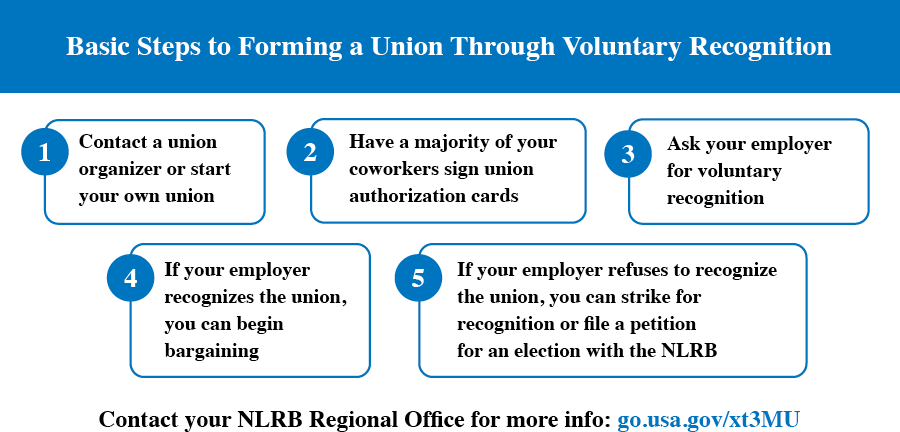
\includegraphics[width=\imageWidth]{images/DOL}
  \captionsetup{justification=centering, singlelinecheck=false, margin=2cm}
  \caption[Forming a Union]{The steps for forming a union or joining an existing union. (Source: US Department of Labor.)}
  \label{fig:DOL}
\end{figure}

If the employer refuses to negotiate, the union can file an “unfair labor practice.” They can also strike or conduct other work stoppages until the recalcitrant employer meets their demands or agrees to negotiate. These are \textit{coercive} strategies that are meant to compel the employer to act or not act in a particular way or to exact concessions. These strategies are also \textit{relatively more conflictual} vis-\`a-vis the Building Trades' approach.

\subsection{Building Trades Bargaining}\label{bt_bargaining}

In contrast to this approach, building and construction trade unions do not usually organize the workers at the workplace. They typically establish voluntary agreements with employers; since these agreements are voluntary, once they expire, the employer has no obligation to continue to bargain with the union. This places the union at a significantly weaker position vis-\`a-vis their bargaining strength and leverage. Since these agreements can be established before any workers are hired,\footnote{The union does not need to organize the workers. The union only needs to convince the employer to \emph{voluntarily} enter into an agreement with the union.} they are called prehire agreements. Prehire agreements have a long history that predates their legitimation by Congress in 1959 when the \acrfull{lmrda} was passed. In fact, before the \acrshort{lmrda}, the \acrshort{nlrb} had refused to take jurisdiction over the building and construction trades because prehire agreements were technically a violation of the \acrshort{nlra} and the agreements would have to be invalidated. Instead, they allowed the construction unions to operate essentially illegally. It was not until the 1959 passage of the \acrshort{lmrda} that the official exception was carved out for construction unions in Section 8(f). So, whereas labor law is often discussed in terms of how it constrains union organizing efforts (i.e., how laws have been "imposed from above"), this is not the case with respect to prehire agreements used by the building and construction trades; they were already organizing this way before the passage of the \acrshort{lmrda}. Put differently, this is not a tragic story of how construction unions were forced to organize conservatively.

Each contract type points to a different orientation toward the boss and approach to mobilizing worker power. Perhaps most notable is the starting point of the unionization process (Figure \ref{fig:organizing_paths}). The "industrial" path (on the left) starts with the employees already hired. Sometimes, the effort is primarily driven by union staff; other times, it can be driven more by shop floor organizers from the rank-and-file. Either way, the approach is to organize workers around issues they are facing in the workplace and compel the employer to negotiate a contract through coercive measures such as strikes or using the state as an instrument to compel the employer to bargain in good faith. The building and construction trade unions largely dispense with this approach; instead, they try to entice employers based on their members’ skill and training and by collaborating with the employers.\footnote{Again, the building and construction trades are not forced by law to organize in this way; it is their choice whether to organize in this way or another way.} This "construction union" path is depicted on the right.

\begin{figure}[ht]
  \centering
  \includegraphics[width=\imageWidth]{images/organizing_paths}
  \captionsetup{justification=centering, singlelinecheck=false, margin=2cm}
  \caption[Union Organizing Paths]{The industrial mode of organizing (left) and the construction mode of organizing (right). Construction unions may follow either path, but other unions may not voluntarily negotiate the way that construction unions can.}
  \label{fig:organizing_paths}
\end{figure}

One practical reason for the development of prehire agreements in the building and construction trades is the temporary nature of the work. Because of the temporary nature of the work, many union halls maintain a hiring hall with dispatch procedures for members out of work. At the completion of the job assignment, laid-off union members may return to the union’s hiring hall and make themselves available for employment somewhere else by signing the out-of-work list maintained by the union. The union will dispatch its members to jobs as needed by the employer. Because of the temporary nature of the job, organizing via the traditional route is much more challenging because workers are laid off frequently, and the employer has no permanent workforce, at least not like other workplaces do. 

From that perspective, prehire agreements are a practical response to the specific unionization challenges faced in the construction industry. However, this particular arrangement has serious consequences for how construction unions must situate themselves in relation to the employer. Because of the voluntary nature of the agreements, the employer may simply choose to leave the collective bargaining relationship at the contract's expiration. Thus, construction unions that follow this method of organizing generally must maintain a much more employer-friendly orientation than unions that organize through the other route. Simply put, if the employer feels that the workers are pushing too hard to enforce their contract or that the union has become too radical, the employer is free to leave at the next bargaining round.

However, the Building Trades have more leverage when the project requires highly-skilled workers because of the sophistication of the job or when the job is so large that the employer cannot sufficiently staff the job without using the union's hiring hall (these often overlap). In other words, a building trades union wields the greatest power when the employer has a sophisticated project that requires highly skilled workers to complete the project successfully. When this is the case, the employer has little choice but to hire union workers (Figure \ref{fig:union_power_red}). Rather than organizing the workers on the shop floor to demand concessions and better working conditions from their employers, construction unions use their leverage as a particularly skilled workforce that employers need to complete their projects. Of course, this also is not absolute. "Highly skilled" is relative to the skill level of the non-union workers (i.e., those without union training). As the nonunion's training improves, and the trade is "deskilled" (i.e., new materials and installation techniques are introduced that are easier to install), the union has to be cautious regarding how strongly it asserts itself and pressures employers. For example, when flexible plastic PEX piping was introduced, which is much easier to install than copper tubing (or galvanized piping, which was popular in the 1950s and 1960s), it threatened the plumbers' union's leverage. Its installation requires little training and no knowledge of soldering techniques. The \acrfull{ua} opposed its introduction because it would deskill installation and fought unsuccessfully against its adoption as an acceptable building material in the California Building Code (\cite{faloonCaliforniaConsumerGroups2002, CaliforniaCaughtDebate2004}). For the \acrshort{ua}, this represents a substantial loss and a victory for the non-union insofar as union training is now less valuable to some extent.

This threat inclines building trades unions to be employer-friendly. For example, the union does not have exclusive control over its training program. Instead, each union has a \acrfull{jatc} that oversees the training process and curriculum development. The \acrshort{jatc} is a committee comprised of 50 percent labor and 50 percent management, each having an equal share in controlling the apprenticeship program. This promotes a greater cohesion between labor and management. From this perspective, the union and management are a team. They have a mutual interest in reproducing each successive generation of union construction workers. Significantly, this requires the union to cede, at least partially, control over the process to the employer. 

\begin{figure}[ht]
  \centering
  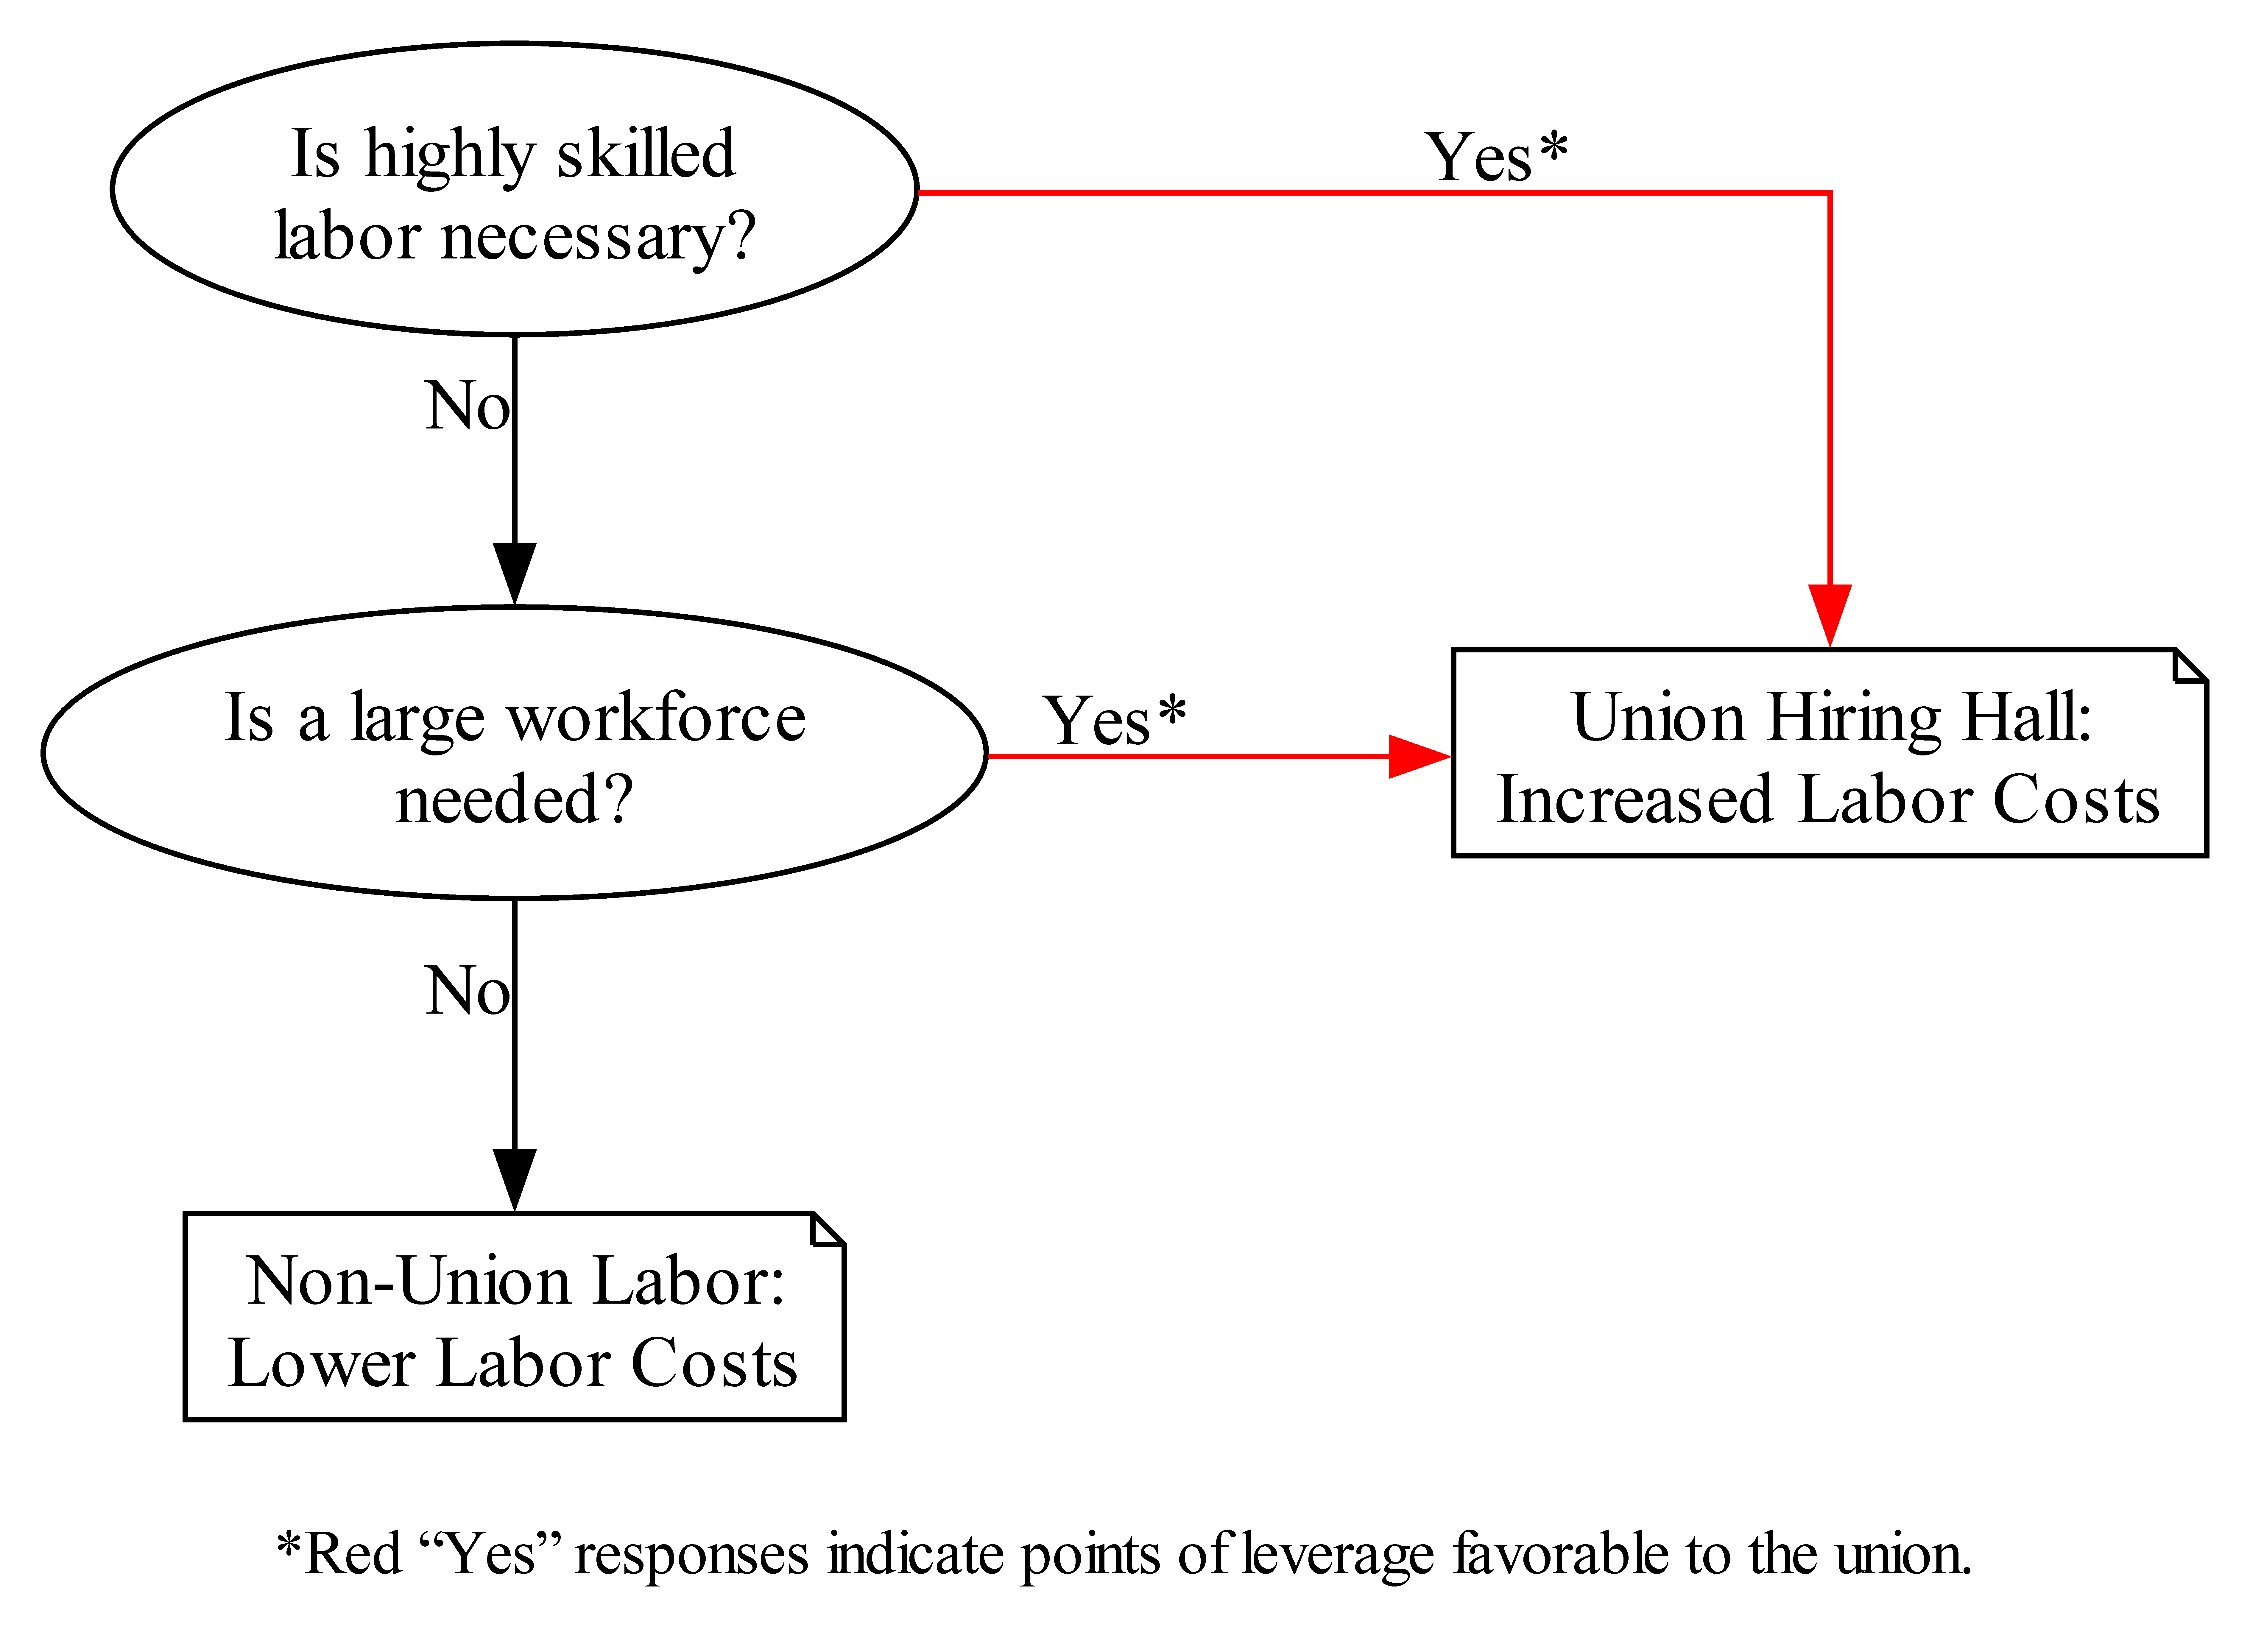
\includegraphics[width=\imageWidth]{images/union_power_red}
  \captionsetup{justification=centering, singlelinecheck=false, margin=2cm} 
  \caption[Union Leverage and Power]{Since negotiations between construction unions and employers are voluntary, construction unions typically have more leverage where the employer requires a more skilled workforce or where the job is large and requires many employees.}
  \label{fig:union_power_red}
\end{figure}

%\subsubsection*{The hiring hall}\label{hiring_hall}

The hiring hall is an integral component of the prehire contract arrangement. Without the hiring hall, the prehire scheme would not be tenable. A skilled "pool of labor" ready to be dispatched is necessary to attract employers and convince them to \emph{voluntarily} sign a prehire agreement. This scheme is well-suited for construction because of the contingent nature of construction work. As Murphy explains:

\begin{quote}
Many construction industry employers hire employees, as the need arises, to work on a particular project and to be laid off when their services are no longer required. Most construction workers are organized into union hiring halls. A hiring hall, or work referral system, is an arrangement under which a union that "has control of or access to a particular labor pool agrees to supply workers to an employer upon request." When an employer in the construction industry needs skilled workers for a project, he often seeks such workers from the union hiring hall. Historically, the practice in the construction industry was for the employer to sign an agreement with the hiring hall union, which set the terms and conditions of employment for workers not yet hired. These contracts, known as pre-hire agreements, often contemplated a tenure of years, spanning several projects. Rather than having to renegotiate the terms and conditions of employment on each new project, the employer was assured a ready supply of skilled workers and predictable labor costs upon which to base his bids on projects subcontracted by a general contractor. Furthermore, construction workers had the benefit of a central clearinghouse for employment opportunities. (\cite[1014–15]{murphyPreHireAgreementsSection1982})
\end{quote}

\noindent{}This configuration, detailed in \autoref{fig:hiring_hall}, is the scheme still used in construction unions to this day,

\begin{figure}[!h]
  \centering
  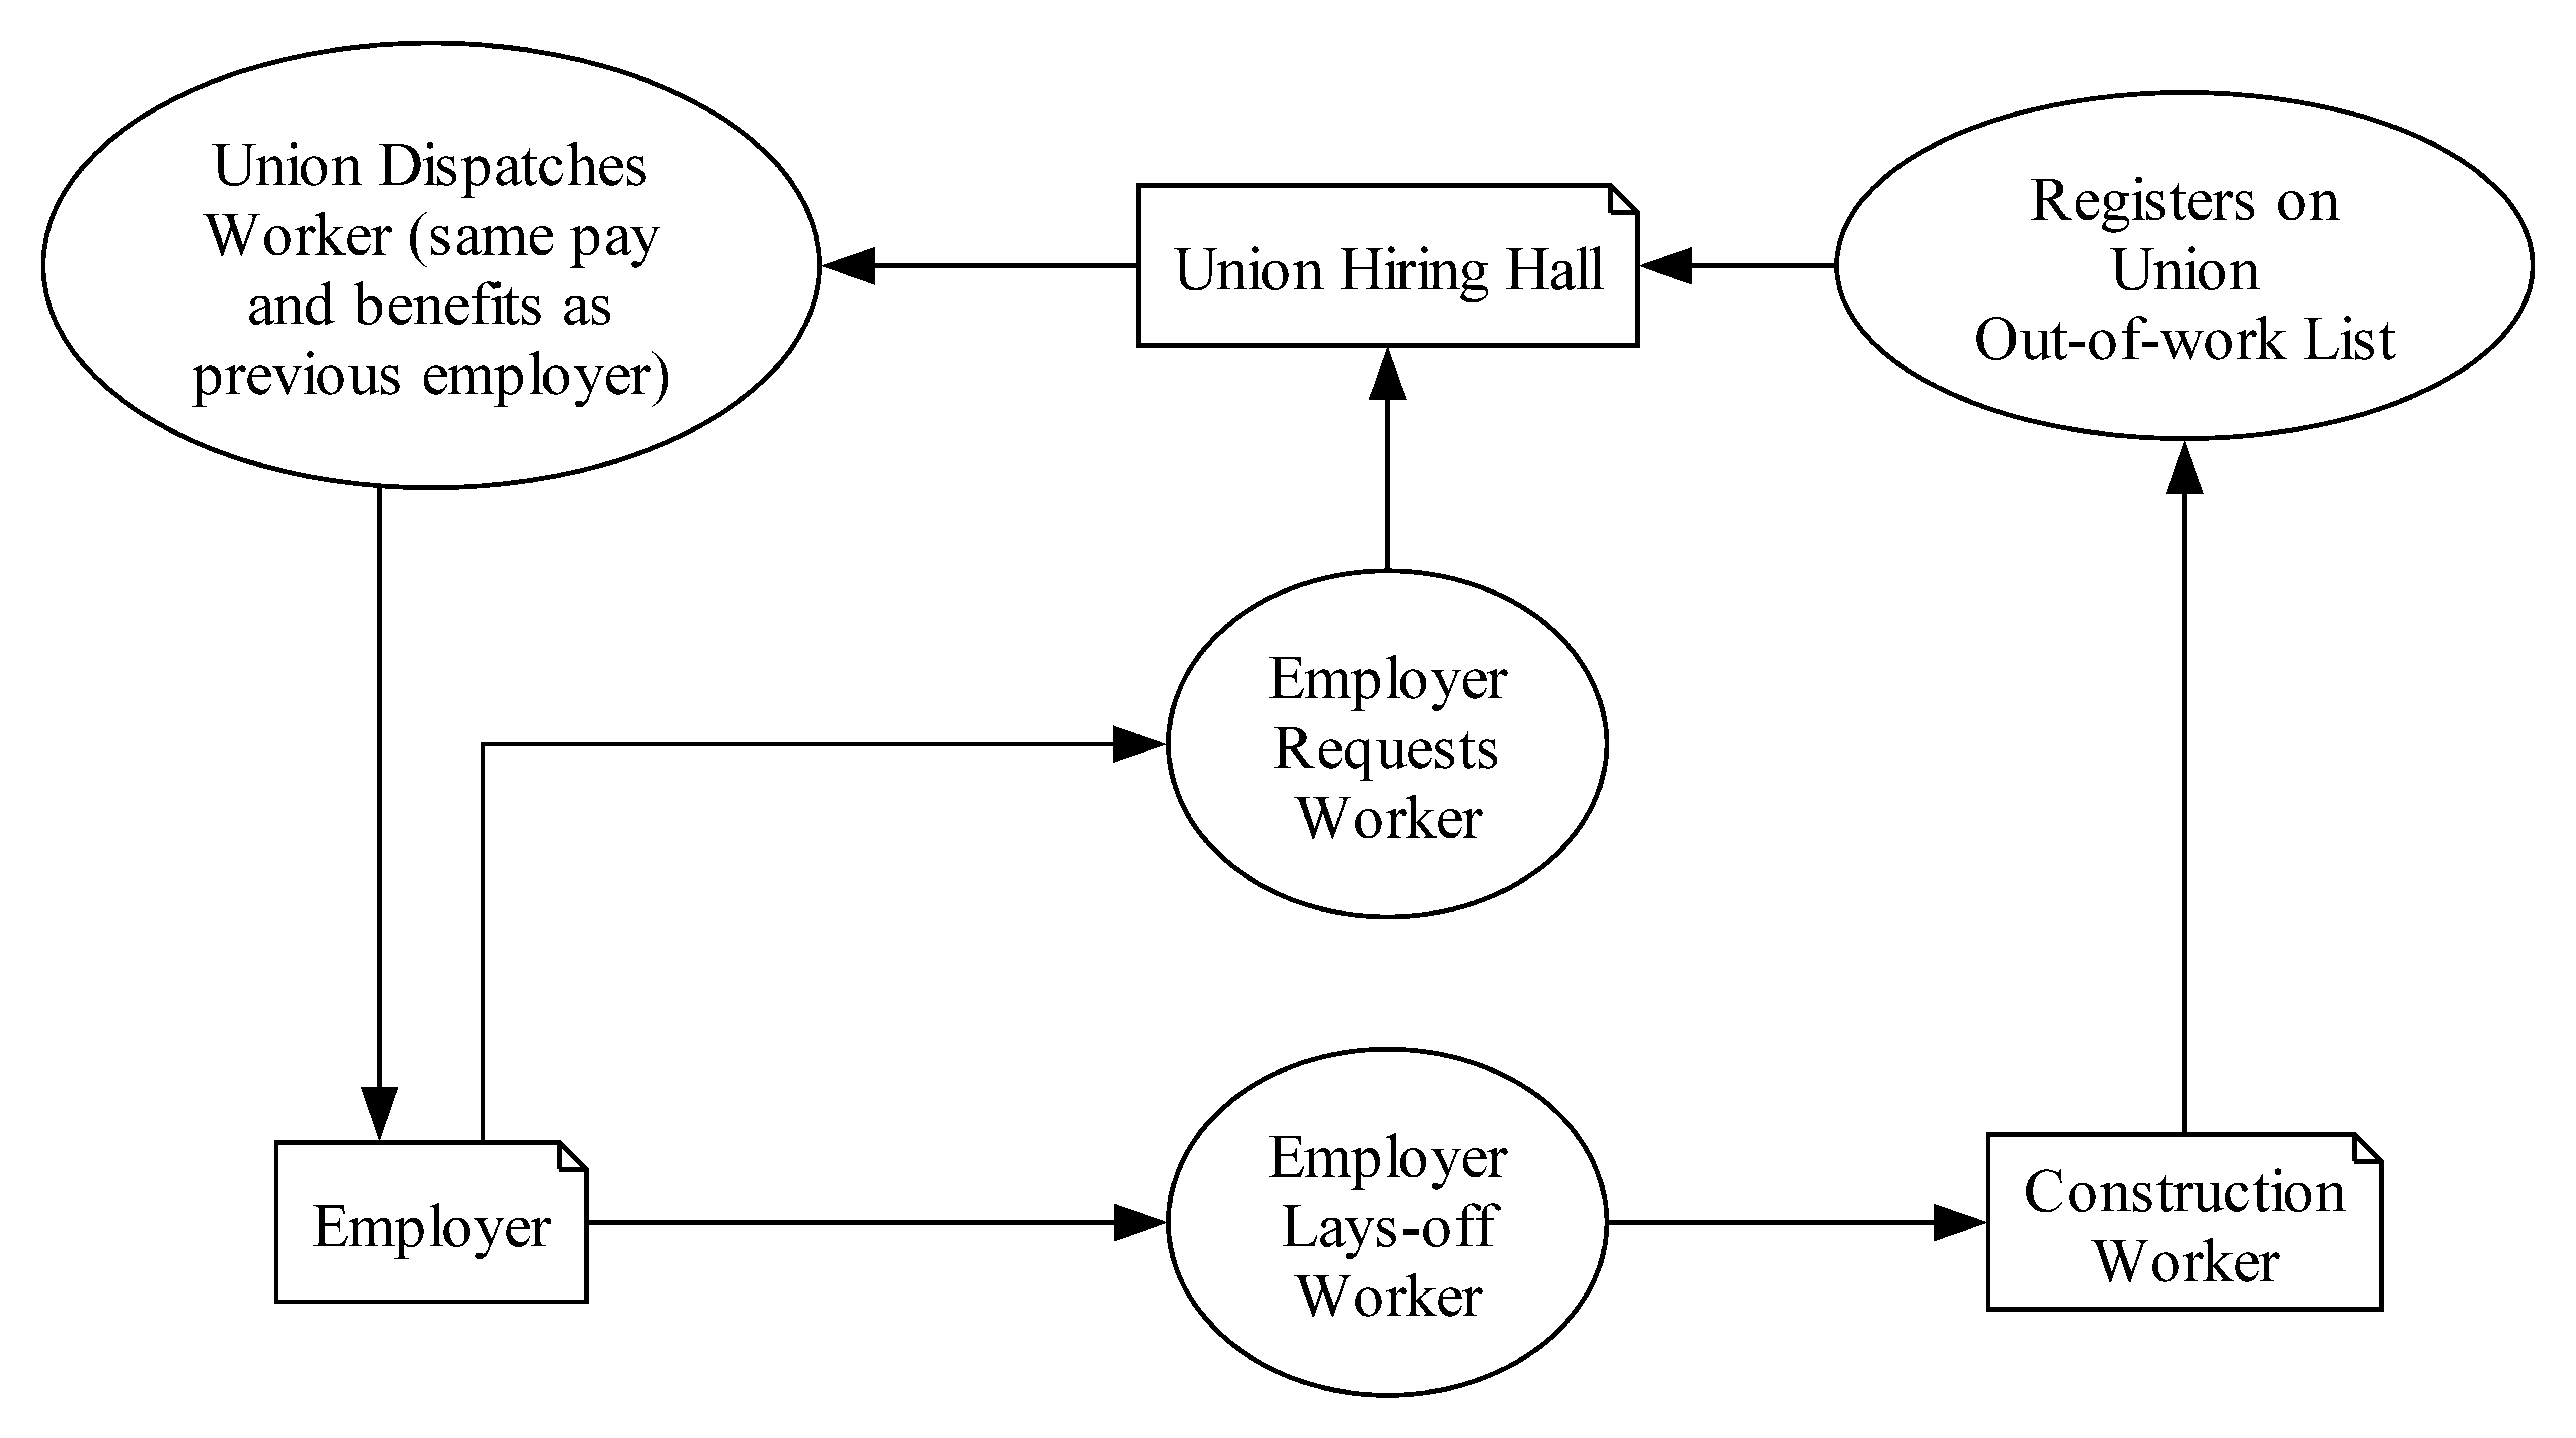
\includegraphics[width=\imageWidth]{images/hiring_hall}
  \captionsetup{justification=centering, singlelinecheck=false, margin=2cm} 
  \caption[Union Hiring Hall]{Construction unions usually maintain a hiring hall. When employers require more workers for their projects, they contact the hiring hall to request workers to be dispatched to the job site.}
  \label{fig:hiring_hall}
\end{figure}

\section{An Outlier in the Labor Movement}\label{outlier}

Unions often find themselves at the crossroads of political and social movements, particularly environmental movements, raising questions about their alliances and priorities. The \acrfull{uaw} could be negatively affected by transitions from fossil fuel burning vehicles to electric insofar as those new plants may not be unionized and it may result in job losses (\cite{feeleyElectricVehicleFactories2023}). The \acrfull{usw} faces more job losses at oil refineries\footnote{Some job losses were already brought on by the pandemic.} if climate policy restricts the operation of those facilities. Building Trades workers face unemployment if pipelines cease to be built and petrochemical refineries are shut down. Despite the contradictions, many labor unions have taken a long-term approach to the problem. They want green, environmentally-friendly jobs that are also good jobs with union wages and benefits. However, the Building Trades unions have not been among those unions.

\subsection{Dakota Access Pipeline and Standing Rock}\label{dapl}

The controversy surrounding the \acrfull{dapl} brought to the fore the political differences vis-\`a-vis the Building Trades' unions on the one hand and the rest of the labor movement on the other. The plan to build a 1,168-mile crude oil pipeline, called the \acrshort{dapl}, stretching from the Bakken and Three Forks production region of North Dakota to Patoka, Illinois, was announced in 2014 by Dakota Access, LLC (\cite{oconnellDakotaAccessPipeline2018, sahaFiveThingsKnow2016, usarmycorpsofengineersDakotaAccessPipeline}). For the first roughly two years after the announcement of the project, it, by and large, did not draw public attention or awareness. However, in the fall of 2016, it became a flashpoint in the national political scene, with environmental groups and Native American tribes on one side and petrochemical companies on the other. 

The opposition to the pipeline culminated in protests in Sioux County, North Dakota in 2016. The pipeline was slated to run through the Standing Rock Sioux Tribe reservation, which opponents of the project contended would “endanger[] sacred sites and drinking water” (\cite{sahaFiveThingsKnow2016}). Members of the Standing Rock tribe claimed that the project violated the principles of tribal sovereignty and threatened the continued existence of the tribe (\cite{massieUnderstandDakotaAccess2016}). Moreover, they claimed that the US government had not adequately consulted with the tribal government, which violated US treaties and the United Nations Declaration on the Rights of Indigenous Peoples (\cite{sahaFiveThingsKnow2016}). In addition to bringing thousands of Native American activists in opposition to the pipeline from across the country to Standing Rock, environmentalists and climate activists were equally concerned not only with the environmental impact of expanding fossil fuel infrastructure but also the potential hazards of oil spills and other accidents endemic to the petrochemical industry (\cite{sahaFiveThingsKnow2016}). 

The Standing Rock Sioux Tribe filed a lawsuit against the US Army Corps of Engineers in an attempt to halt the project. On September 9, 2016, a federal judge denied the tribe’s request to halt construction. However, within hours of the court’s ruling, the Obama Administration ordered the Army Corps of Engineers to put the project on hold and “determine whether it will need to reconsider any of its previous decisions regarding the Lake Oahe site under the \acrfull{nepa} or other federal laws” (\cite{officeofpublicaffairsJointStatementDepartment2016}). 

%\subsubsection*{Organized labor's response}

Many labor organizations supported the Native tribe and the environmentalists. For example, the \acrfull{seiu} emphasized that more than jobs were at stake; the pipeline would threaten the health and safety of “low income communities and communities of color, including those where many \acrshort{seiu} members live and work” (\cite{nlfUnionsWeighDakota2016}). Other unions, including the National Nurses United and the Communication Workers of America, also expressed these solidarities with environmental and other movements (\cite{nlfUnionsWeighDakota2016}). Additionally, an entire coalition of trade unions and labor groups, the \acrfull{lcca}, collectively issued a statement opposing the pipeline. This coalition includes the A. Phillip Randolph Institute, the Asian Pacific American Labor Alliance, the Coalition of Black Trade Unionists, the Coalition of Labor Union Women, the Labor Council for Latin American Advancement, and Pride at Work (\cite{apalaAFLCIOConstituencyGroups2016}).

The group emphasized how labor’s interests are not at odds with environmental and Native American concerns and interests:

\begin{quote}
We remain committed to fighting the corporate interests that back this project and name this pipeline “a pipeline of corporate greed.” We challenge the labor movement to strategize on how to better engage and include Native people and other marginalized populations into the labor movement as a whole. (\cite{apalaAFLCIOConstituencyGroups2016})
\end{quote}

\noindent{}However, the \acrshort{lcca} also recognized that simply shutting down the construction of the pipeline would not be sufficient; the creation of good jobs to replace the ones lost by halting the pipeline’s construction was necessary:

\begin{quote}
Lastly, we applaud the many labor unions working to create a new economy with good green jobs and more sustainable employment opportunities for all. We also encourage key stakeholders — labor unions including the building trades, the Standing Rock Sioux tribe and others who would be impacted — to come together to discuss a collective resolution. (\cite{apalaAFLCIOConstituencyGroups2016})
\end{quote}

\noindent{}Lastly, the \acrshort{seiu} released a statement that emphasized the importance of both good jobs \emph{and} the environment. The statement is remarkably similar to the \textit{Just Transition} idea that the \acrfull{ocaw} first crafted decades earlier and that the \acrfull{usw} still embraces today:\footnote{The \acrshort{usw} is a union that both has many workers in the petrochemical industry \emph{and} supports green energy policy. They even support ceasing operations of many of the plants that their members work in as part of that commitment. This is discussed at greater length in \fullref{ocaw}.}

\begin{quote}
\acrshort{seiu} members recognize the importance of these jobs for these workers and their families and we demand that our government protect all workers whose lives and livelihoods are impacted by a shift away from fossil fuels. Our government must make the needed investments into building a new clean economy, including a just transition of workers from the fossil fuel workforce, by investing in clean energy and rebuilding and repairing much of our nation’s aging infrastructure, including existing pipelines which are in great need of repair. We will fight for an economy and democracy in which working families can live and work in a clean environment with good jobs for all. (\cite{nlfUnionsWeighDakota2016})
\end{quote}

The \acrshort{seiu} and other unions opposed to the pipeline were engaged in a collective struggle against the company that planned to build a pipeline through the community, polluting the land and water without any respect to indigenous groups, such as the Standing Rock Sioux. The \acrshort{lcca} made clear in its statement that it was against the "corporate greed" that the project represented (\cite{apalaAFLCIOConstituencyGroups2016}).

%\subsubsection*{The Building Trade's response}

\glsentrylong{nabtu}, a trade department of the \acrshort{aflcio} representing 14 constituent building trades unions, issued a statement within days condemning the actions of the Obama Administration. On September 14, 2016, they expressed their “disappointment” with the Obama Administration in the latter’s willingness to “halt the lawful construction” of the \acrshort{dapl}, emphasized the advanced training of their skilled craftworkers, and contended that many safety redundancies would be in place while the project was underway  (\cite{nabtuStatementObamaAdministration2016}). Further, they chided the Executive Branch for its “disregard” of “the facts,” the “exhaustive permitting and review process, stakeholder engagement,” and “the ruling of a Federal Court Judge,” and they lamented the loss of construction jobs with “family sustaining wages and benefits” (\cite{nabtuStatementObamaAdministration2016}).

Early the following month, the \acrshort{nabtu}, with signatures from the presidents of five construction unions, wrote a letter directly to the White House reiterating their concerns. In the letter, they underscored that many of their 8,000 members who were working on the project were already struggling and facing hardship because of unemployment caused by the Executive Branch’s intervention. Additionally, they emphasized that this intervention sets a “chilling” precedent that would undermine “future investment in necessary U.S. infrastructure---from highways and bridges to ports and factories,” and that “If companies like Energy Transfer Partners cannot trust that the regulatory process outlined in federal law will be upheld, who will continue to invest in America?” (\cite{callahanLetterObama2016}).

\section{Union Members as Shareholders}\label{union_shareholders}

The \acrshort{nabtu} has clearly taken a very different position than the rest of organized labor. But why are the building trades taking such a different stance? One might think that they also would be guided by a broader notion of unionism; after all, their members also live and work in the communities that are being harmed by global warming. That is, the ranks of these unions are also, often enough, comprised of the same people that the \acrshort{lcca} and unions like the \acrshort{seiu} are defending from being harmed by the pipeline. What principles guide this sort of unionism?

A 2015 interview with Sean McGarvey, President of \acrshort{nabtu}, provides some answers. McGarvey met with Martin Durbin, President and CEO of \acrfull{anga} for an interview later released on YouTube. At one point, Durbin talked about his time on the American Petroleum Institute’s labor-management board in Pennsylvania. Durbin explained that when the industry moved into Pennsylvania, labor and management did not have an existing relationship, but eventually they found that, according to Durbin, their interests overlapped and that both sides mutually benefitted from the relationship:

\begin{quote}
Pennsylvania, I thought, was a really interesting example where we saw an industry move in and where the [labor-management] relationship didn't really exist but over time everyone kind of realized that, hey, wait a minute, you know, this is working for all of us. (\cite{natgasnowNextInfrastructureChallenge2015})
\end{quote}

\noindent{}When Durbin asked McGarvey how he thought these relationships with management had been progressing, McGarvey responded:

\begin{quote}
It’s really been interesting to work on building these relationships. We have so much in common as opposed to the things we disagree with, and we've gotten together and said, “Let's really examine these things we have in common”; and then once we examine them we said, “Well, how do we partner to move the issues along that we really agree with that are in the best interest of our country and our economy?” And [we’ve had] the opportunity to work with really smart people in really iconic great companies that have been around for a hundred years or have been around for 20 years\ldots{}I serve a membership; my job is to create economic opportunity for my membership\ldots{}That's what I'm supposed to do and when you run a company, you have a board of directors, and you have shareholders to answer to if you're if you're publicly traded. Both of those things are true, but then there's this meeting in the middle: how do we create value for shareholders? How do I create value for my members and do it in a responsible way working with partners who want to work with us responsibly to create value for their shareholders?\ldots{}[W]hen you have the opportunity to have those conversations you say, “gosh there [are] so many things that we can do together and do better together,” and I [have] got to tell you\ldots{}it's always kind of been the way [of] the building trades. If you go back to a great quote from George Meany, back when he was a plumber in New York City and a local leader, they never went on strike; they never had a strike, even during that tumultuous time down there. It's because [the union’s] contractors needed to be successful for his plumbers to work. (\cite{natgasnowNextInfrastructureChallenge2015})
\end{quote}

\sloppy
McGarvey’s answers exemplify the class collaborationist approach taken by the \acrshort{nabtu}. Contra other unions, the \acrshort{nabtu} has prioritized its relationship with industry over solidarities with the Native American tribes and environmental groups. McGarvey made very clear that he thinks the building trades should prioritize their relationships with management by finding the things that they have in common over policies that might benefit workers or the community more broadly. The analogy of Building Trades leader to essentially a CEO is equally telling. From this perspective, the union members become not much more than “shareholders,” who pay dues and other fees in exchange for a “return” in the form of employment covered by a collective bargaining agreement. Rather than these agreements being forged as a result of workplace organizing, where work stoppages or other such actions are the crux of such struggles, they are forged in labor-management board meetings, where the parties find ways to collectively create “value” for their shareholders or members. Indeed, as the George Meany reference makes clear, strikes are rare to nonexistent by design.
\sloppypar

Of course, strikes are rare in general, but as a relative measure they are even less frequent in construction. In 2022, 14.3 million workers were unionized; about 3 million (20.9 percent) of them work in construction (\cite{blsUnionMembersSummary2024}). That same year, there were 413 labor actions, such as strikes or other work stoppages, but only three were in the construction industry (0.73 percent), meaning that 99.3 percent of labor actions were outside of the construction industry (\cite{ilrschoolILRLaborAction}). This is about one-tenth the “expected rate” if construction workers had labor actions at a rate equal to their proportion of the unionized workforce. That is, strike activity, as rare as it might be, is coming disproportionately from non-construction sectors (Table \ref{tab:strikes}).

\begin{table}[h]
\centering
\begin{tabular}{llll}
                    & All            & \multicolumn{2}{l}{Construction} \\ \hline
Unionized Workforce & 14.3 million	& 3 million				& 20.9 \%     \\
Labor Actions       		& 413				& 3							& 0.73 \%    
\end{tabular}
\captionsetup{justification=centering, singlelinecheck=false, margin=2cm} 
\caption[Labor Actions]{Construction unions represent nearly 21 percent of unionized workers but were involved in less than one percent of labor actions in 2023 (\cite{ilrschoolILRLaborAction}).}
\label{tab:strikes}
\end{table}

It is also true that class collaboration is not limited to petrochemical work, and that the building trades could at least in theory choose class collaboration with green industry. But this would only be possible if the green energy industry had a reason to collaborate in the first place. Recall that construction collective bargaining agreements are voluntary, and that construction employers usually only have an incentive to sign these agreements if their jobs require highly skilled labor or if they would benefit from the quick deployment of a large number of workers. Green energy companies have, by and large, been able to build without union labor (\cite{scheiberBuildingSolarFarms2021}), suggesting that they either do not need these things or have been able to obtain them elsewhere (which would mean that the union is losing its monopoly of these commodities). So, there is no reason for those employers to pay union wages and into union benefits and pension funds if they don’t need to. Simply put, green energy has largely not needed construction unions, and thus, construction unions have largely failed to make inroads in green energy.

\section{Comparing the building trades with other unions}\label{interunion_cases}

I selected two cases that share similar features with the building and construction trades for comparison: the \acrlong{ocaw} (\acrshort{ocaw}; now part of the Steelworkers [\acrshort{usw}]), a union that has many members working in the petrochemical industry, and the \acrfull{iam}, a craft union that does not organize workers the way that the building trades unions do.

%Also, an intra-building trades union comparison is made between the general building trades orientation and those building trades unions who have chosen to conduct \acrshort{nlrb} elections in the same way that non-construction unions do.

% Is this the best place to put this specific case?
\subsection{The United Association of Plumbers and Pipe Fitters (UA) Local 189}\label{ua_189}

I chose \acrfull{ua} Local 189 in Columbus, Ohio because of the \acrfull{ua}'s large amount of pipeline and petrochemical refinery work. I relied on Richard Schneirov's \textit{Pride and Solidarity} for historical background on Local 189. Though it focuses specifically on Columbus, it is situated in the broader craft union developments of the time. Because both the \acrfull{usw}/\acrfull{ocaw} share a large amount of petrochemical work, this made Local 189 an ideal comparative case.

In his masterful study of the United Association of Plumbers and Pipe Fitters (\acrshort{ua} Local 189 in Colombus, Ohio, Richard Schneirov (\citeyear{schneirovPrideSolidarityHistory1993}) details the uniqueness of construction unionism. The formation of the \acrshort{ua} began in the late 1880s; before then, plumbers and pipe fitters were largely unorganized; to the extent that they did form unions, the organizations were usually temporary, to meet a specific need at a particular time and were hyper-local and fragmented, without any international\footnote{A term that, in the context of US and Canadian unions, means a national organization.} to push for the interests of plumbers and pipe fitters across the nation (\citeyear[58]{schneirovPrideSolidarityHistory1993}). The first boon for the pipe tradesmen was not an organizing campaign undertaken by the union but the American Federation of Labor’s (\acrshort{afl}) eight-hour-day movement (\citeyear[11, 43–45]{schneirovPrideSolidarityHistory1993}). Many pipe tradesmen in the late 1880s and early 1890s worked upwards of ten hours a day, sometimes up to fourteen hours per day. This movement was extremely important because "Hitherto, [unions] had only been able to mobilize large groups of workers for short periods of time" (\citeyear[43–45]{schneirovPrideSolidarityHistory1993}). It also broadened solidarities, appealing to workers of "all natalities, races, trades, industries, skills levels, and genders" (\citeyear[43]{schneirovPrideSolidarityHistory1993}). Though the eight-hour-day movement was largely associated with unionism, which provoked strong resistance from employers, it even appealed to non-union workers (\citeyear[45]{schneirovPrideSolidarityHistory1993}). From that perspective, it was also able to "cement union sentiment and loyalty among large numbers of nonunion workers" (\citeyear[45]{schneirovPrideSolidarityHistory1993}). And in contradistinction to earlier union efforts, this brought unions together across the nation, culminating in a nation-wide eight-hour-day strike on May 1, 1886. However, three days later, the movement suffered a significant setback when anarchists bombed the Haymarket Square in Chicago, killing seven police officers (\citeyear[45]{schneirovPrideSolidarityHistory1993}).

Yet, the eight-hour movement’s efforts proved to be more durable, and on November 15, 1889, it gave rise to the formation of the first union of journeymen plumbers and pipe fitters Local 5180 in Columbus (\cite[45]{schneirovPrideSolidarityHistory1993}). In 1890, Columbus streetcar workers continued to push for shorter workdays. They demanded a reduction from ten to nine work hours per day. In this context, the plumbers and pipe fitters were well positioned to exact concessions from the master plumbers because of fears that the latter could not defeat the former (\citeyear[45–46]{schneirovPrideSolidarityHistory1993}). The master plumbers agreed to a reduction in work hours without a loss in pay. However, the Local was inexperienced in negotiations with the master plumbers, and they were willing to make their concessions to the employers that would allow the latter to severely restrict the time when overtime pay would start (\citeyear[46–47]{schneirovPrideSolidarityHistory1993}). The union sought the advice of the \acrshort{afl} founder Samuel Gompers, who disabused the local union from making concessions (\citeyear[46–47]{schneirovPrideSolidarityHistory1993}). The two sides eventually reached a written agreement, the first of its kind in the trade. 

This encouraged the formation of the city’s first \acrfull{btc}. Despite earlier challenges in uniting the trades, the Council brought all crafts together: bricklayers, lathers, painters, carpenters, tinners, and plumbers and pipe fitters, under the banner popularized by the Knights of Labor: "An injury to one is the concern of all" (\cite[47]{schneirovPrideSolidarityHistory1993}). And notwithstanding the master plumber’s earlier concessions, this inter-union trade solidarity set the stage for even more militancy. The \acrshort{btc} opted, in the words of the Columbus Dispatch, "for ‘radical measures’ at the opening of the ensuing building season" (\citeyear[47]{schneirovPrideSolidarityHistory1993}). They demanded that union workers, no matter the craft or trade, perform the work on every union job site (\citeyear[47]{schneirovPrideSolidarityHistory1993}). If their demand was not honored, the \acrshort{btc} threatened not to "touch any job" where non-union workers were present. Simply put, this meant that if one craft were union on a job site, union workers on the site would refuse to work there unless every other craft was also unionized.

But by 1892, the union had pivoted to issues concerning the integrity of the craft. The union framed the integrity of the craft in the language of public health. The Columbus Trades and Labor Assembly contended that "nearly all the houses that are built for renting purposes are fitted with bad plumbing causing disease and death" (\cite[47–48]{schneirovPrideSolidarityHistory1993}). In response to these issues, the Assembly pushed for the city to adopt building codes and endorsed a union plumber for city inspector (\citeyear[48]{schneirovPrideSolidarityHistory1993}). In addition, the union began to place greater emphasis on the development of an apprenticeship program; the union asked the master plumbers for another raise and the establishment of an apprenticeship program "governing the number and conduct of apprentices" (\citeyear[48]{schneirovPrideSolidarityHistory1993}). The master plumbers refused, and the union went on strike. The master plumbers brought in strikebreakers, and the union eventually lost.

But the plumbers and pipe fitters union had not entirely abandoned broader solidarities. They continued to be involved in the BTC and the Trades and Labor Assembly in an effort to "advanc[e] labor’s political strength" (\cite[50]{schneirovPrideSolidarityHistory1993}). One leader, Louis Bauman, epitomized the class-based orientation of the era. Bauman was the vice president of the Trades and Labor Assembly in 1893, and, beginning in 1894, he also served as the president of Local 57 of the plumbers and pipe fitters. He "was a Labor-Populist, aligned with radical farmers in the Farmers’ Alliances and the National People’s party and with the union men who felt that something should be done to change an economic system in which workingmen were impoverished while Wall Street banks and national corporations dominated the government" (\citeyear[50]{schneirovPrideSolidarityHistory1993}). The Columbus Trades and Labor Assembly’s 1894 constitution exemplified its radical principles:

\begin{quote}
It is self-evident that, as the power of capital combines and increases, the political freedom of the masses becomes more and more a delusive force. There can be no harmony between capital and labor under the present industrial system for the simple reason that capital, in its modem character, consists very largely of rent, interest, and profits, extorted from the producers, who possess neither the land nor the means of production, and are therefore compelled to sell their labor and brains or both to the possessor of the land and means of production at such prices as an uncertain and speculative market may allow. Organization of Trades and Labor Unions is one of the most effective means to check the evil outgrowths of the prevailing system. (\cite[50]{schneirovPrideSolidarityHistory1993})
\end{quote}

However, the radicalism of the nascent pipe trades union was fraught with contradictions. In the early 1890s, the union had moved to exclusive agreements. These agreements offered lucrative benefits to entice the master plumbers into a contract. It not only limited the smaller firms’ ability to compete with the master plumbers by requiring union plumbers and fitters to work exclusively for the master plumbers, but it also precluded workers from "handl[ing] any materials not purchased by their immediate employers" (\cite[54]{schneirovPrideSolidarityHistory1993}). In exchange, the master plumbers agreed to allow "the union to set standard rates for the trade," and "offered local unions benefits that they had great difficulty winning otherwise: a closed shop, the eight-hour day, and stable or increased wages" (\citeyear[54]{schneirovPrideSolidarityHistory1993}). At the same time, these agreements undercut the union’s bargaining power and leverage and, in many ways, the interests of union members. In particular, it limited employment opportunities for union members because non-signatory contractors could not employ union members even when paying union wages and adhering to union rules; this also hindered "the freedom of action of the unions" (\citeyear[54]{schneirovPrideSolidarityHistory1993}). Eventually, the contractors’ demands undercut the union’s power so much that the union abandoned the practice of exclusive agreements in 1899 (\citeyear[54–55]{schneirovPrideSolidarityHistory1993}).

Ironically, the abandonment of these exclusive agreements did not trigger union militancy or radicalism, and by the early 1900s, the union had all but entirely abandoned any commitment to improving working conditions; significantly, they also abandoned the broader labor solidarities that had defined the earlier period (\cite[51–54]{schneirovPrideSolidarityHistory1993}). If one word were to characterize this period, it would be "stability." Many unions in the late 1800s were temporary organizations. Indeed, as Schneirov observed, the telephone book and the \acrshort{ua}’s official journal suddenly ceased to list Columbus \acrshort{ua} Local 57 in 1898; it had completely disappeared without any historical record of what precipitated its collapse  (\citeyear[51]{schneirovPrideSolidarityHistory1993}). To achieve stability, American craft unions, following in the tradition spearheaded by the British craft unions, raised their union dues and implemented a quasi-welfare state. At the time, there was no "social safety net" provided by the government, no unemployment benefits, no workers' compensation, no social security benefits, and no Medicare or Medicaid. 

With increased dues, unions were able to finance these benefits and, consequently, keep construction workers in the union much longer than they had previously (\cite[59]{schneirovPrideSolidarityHistory1993}). The Columbus Plumbers and Pipe Fitters Union could also afford to hire professional staff and leadership for the first time. The union hired full-time business agents, who served as "walking delegates," policing the job sites for contract violations and craft jurisdictional violations by the employers (\citeyear[60]{schneirovPrideSolidarityHistory1993}). The business agent was also an organizer, enrolling new members and "pulling a job" if he could not resolve a workplace dispute through negotiation (\citeyear[60]{schneirovPrideSolidarityHistory1993}). And though most employers did not utilize it, in November 1907, the union established a hiring hall as an institution that would later become a staple of construction unionism; the hiring hall required laid-off members to provide the business agent their names so that he could register them on the list of unemployed members and dispatch them, beginning with the first member laid off to the member most recently laid off, at the employers request (\citeyear[60–61]{schneirovPrideSolidarityHistory1993}). Finally, this era ushered in intra-craft solidarity: plumbers and fitters, for the first time, began to see themselves not as individuals trying to "better themselves in the marketplace," hoping not to ultimately become independent masters, but as workers with shared interests with other plumbers and fitters (\citeyear[61]{schneirovPrideSolidarityHistory1993}). These developments made the union into a more durable institution.

\subsubsection*{A contemporary view}

Many elements of fin-de-si\`{e}cle pipe trades unionism are still present in many construction unions today. Schneirov (\citeyear{schneirovPrideSolidarityHistory1993}) contends that the plumbers and pipefitters have had to balance between two sometimes contradictory identities. One is that they are workers with a set of common class interests with other workers in a labor movement built around solidarity for "union brothers and sisters." But from another perspective, they are part of a craft community that values craftsmanship and that takes pride in its work, a value that they share with their employer (\cite[3--4]{schneirovPrideSolidarityHistory1993}). A construction journeyworker is distinct in this regard from other blue-collar workers, such as factory workers on an assembly line, who do a repetitive task that can be easily taught (\cite[5]{schneirovPrideSolidarityHistory1993}). Before one can become a journeyworker, one must complete an apprenticeship, which requires learning how to apply general plumbing and pipe fitting installation techniques, principles, and codes to specific circumstances. This requires a rigorous training program to prepare apprentices for their careers. As a consequence, these workers have gained prestige and a sort of elite status that many other blue-collar workers could only dream of.

At the same time, this elite status and craft pride also come with a much higher degree of collaboration and a much closer relationship with the boss. In fact, in Local 189, as is the case with many other plumber locals across the country, the line could be blurred between employer and union member. Some union collective bargaining agreements even allow for contractors, that is, the owners of the enterprises, to work on projects alongside union employees (\cite[5]{schneirovPrideSolidarityHistory1993}). This is also the case with \acrshort{ua} Local 342 in the San Francisco Bay Area. Local 342 allows employers no more than one owner of the company to "work with the tools," so long as "the Individual Employer has not more than two (2) journeymen and one (1) apprentice dispatched" (Local 342 MLA). Many of these employers who also work "work with the tools" are members of the union. For example, Brown 3 Plumbing in Oakland, California, is owned by William Brown, a Local 342 member who also works on many of his company’s projects (\cite{brownplumbingExecutiveSummary}). LJ Kruse Company in Berkeley, California, similarly has members of the Kruse family who also work on the job site. Will Kruse has completed both the 5-year apprenticeship and serves as the company’s Vice President and Service Manager (\cite{ljkruseUs}). He can be seen on the company’s website donning construction gear with a dirty high-visibility vest and jeans and on a job site with a pile of steel framing in the background. At Local 159 in Martinez, California, Brian Lescure, part of the Lescure family that owns Lescure Company, is both the Union’s Apprenticeship Coordinator and elected to the Union’s Examining Board (\cite{lescureLinkedIn}).

This overlap can give workers a sense, much more so than in other industries, that both employer and employee are on the same "team." Unlike an industry such as manufacturing, where large amounts of capital are necessary to start a business, starting a plumbing business is not unrealizable. One survey even found that half of a large plumbers local "had thought of entering business on their own at one time or another, though most had not done so" (\cite[5]{schneirovPrideSolidarityHistory1993}). Put straightforwardly, this means that half of the local union’s workers, that is, sellers of labor power, also imagine a future as buyers of that same labor power. Schneirov contends that this blurring of the lines and class collaborative dynamic creates a "craft community," where employers and workers share a common background that "breed[s] an ethic of cooperation among individuals based on mutual respect for craft knowledge, skill, and ingenuity" (\cite[6]{schneirovPrideSolidarityHistory1993}). And "Even those union members who have never considered contracting have often bid independently on small jobs and are familiar with the psychology of being an entrepreneur" (\cite[5--6]{schneirovPrideSolidarityHistory1993}). 

\subsection{The Oil Chemical and Atomic Workers \& United Steelworkers}\label{ocaw}

The United Steel Workers (\acrshort{usw}) and the Building Trades both have substantial work in the petrochemical industry. This makes the \acrshort{usw} an ideal comparative case to analyze whether or not unions simply stand behind their employer when threatened with job loss. Recall that the \acrfull{ua} stood behind the petrochemical pipeline companies when the \acrshort{dapl} protests threatened their jobs. The \acrshort{usw}, however, has taken a much different approach with respect to climate change issues and has even advocated for plans that would destroy many of their jobs, so long as workers a protected by the \textit{Just Transition} program that would ensure that they find other employment and are protected by a generous social safety net.

The \acrfull{ocaw} represented workers in the petrochemical industry for much of the 20th Century, but by the 1980s, membership numbers began to decline significantly. They merged with several other unions to form the \acrfull{pace} in 1999. However, that merger only lasted six years, and they merged with the \acrshort{usw} in 2005.

The \acrshort{ocaw} was much more radical than other unions. As Mark Dudzic, a former leader and retired member, once described it, "The oil industry never really accepted the union as a junior partner. The union was never able to win the union shop and all the other accouterments of class peace. As a result, the culture of militancy was deeply embedded in the union" (\cite{leopoldManWhoHated2007}). Though the \acrshort{ocaw} is now dissolved and has gone through two mergers, it is worth tracing the history to the present day to analyze if their radical history has had any lasting effect and if the lack of class peace persists.

Unlike the Building Trades, the \acrshort{usw} is currently a supporter of the Labor for Single Payer Health Care campaign, which is a broad social-wage political effort. From that perspective, the \acrshort{usw} is not just focusing singularly on its members’ interests but is instead committed to broader political struggles. Strikingly, the \acrshort{usw} even supports a transition from dirty-energy to clean-energy jobs. This is significant for a union that has many workers in the petrochemical industry. Such a transition would end their employment at oil refineries and require a new, more challenging struggle to establish a union foothold in new clean-energy sectors, sectors that have been highly resistant to unionization. Nevertheless, the \acrshort{usw} has adopted a broader, more long-term vision, one much more solidaristic with other environmental activist groups than the Building Trades have.

\subsubsection*{OCAW and Tony Mazzochi}\label{mazzochi}

Les Leopold, in \textit{The Man Who Hated Work but Loved Labor}, recounts the story of Tony Mazzocchi, former long-time \acrfull{ocaw} official and organizer. In looking at the history of this union with Mazzocchi as the protagonist, Leopold highlights the social unionism that the former helped craft in the postwar period in New York (\cite[16]{leopoldManWhoHated2007}).

Mazzocchi started his employment at Helena Rubinstein Incorporated on May 1, 1950. Union leaders of the left-leaning District 65 had recruited Mazzocchi to raid an anti-communist \acrshort{cio} union. At the time, District 65 was the largest left-leaning union in New York City. It had disaffiliated with the \acrfull{rwdsu} in August 1948 after the national union had ordered the District to comply with the Taft-Hartley Act (\cite{leopoldManWhoHated2007}), an act passed in 1947 that substantially gutted the Wagner Act and imposed onerous burdens and restrictions on labor unions, severely curtailing their power, so much so that it was commonly denounced by labor as the "Slave Labor Bill" (Figure \ref{fig:slave_labor_bill}). The District 65 leaders were Communist Party members or sympathizers and wanted Mazzocchi to obtain employment at a unionized New York City cosmetics plant, Helena Rubinstein Incorporated, as a "colonizer." His role would be to organize a progressive cadre within the rank-and-file of the Gas, Coke, and Chemical Workers \acrshort{ugccwa} local union, which was present at the plant (\cite[71]{leopoldManWhoHated2007}). They wanted him to work his way up through the leadership ranks and bring the local into the left-leaning District 65. Mazzocchi was hired in May 1950, and through this effort, Mazzocchi got his start as a union organizer.

\begin{figure}[ht]
  \centering
  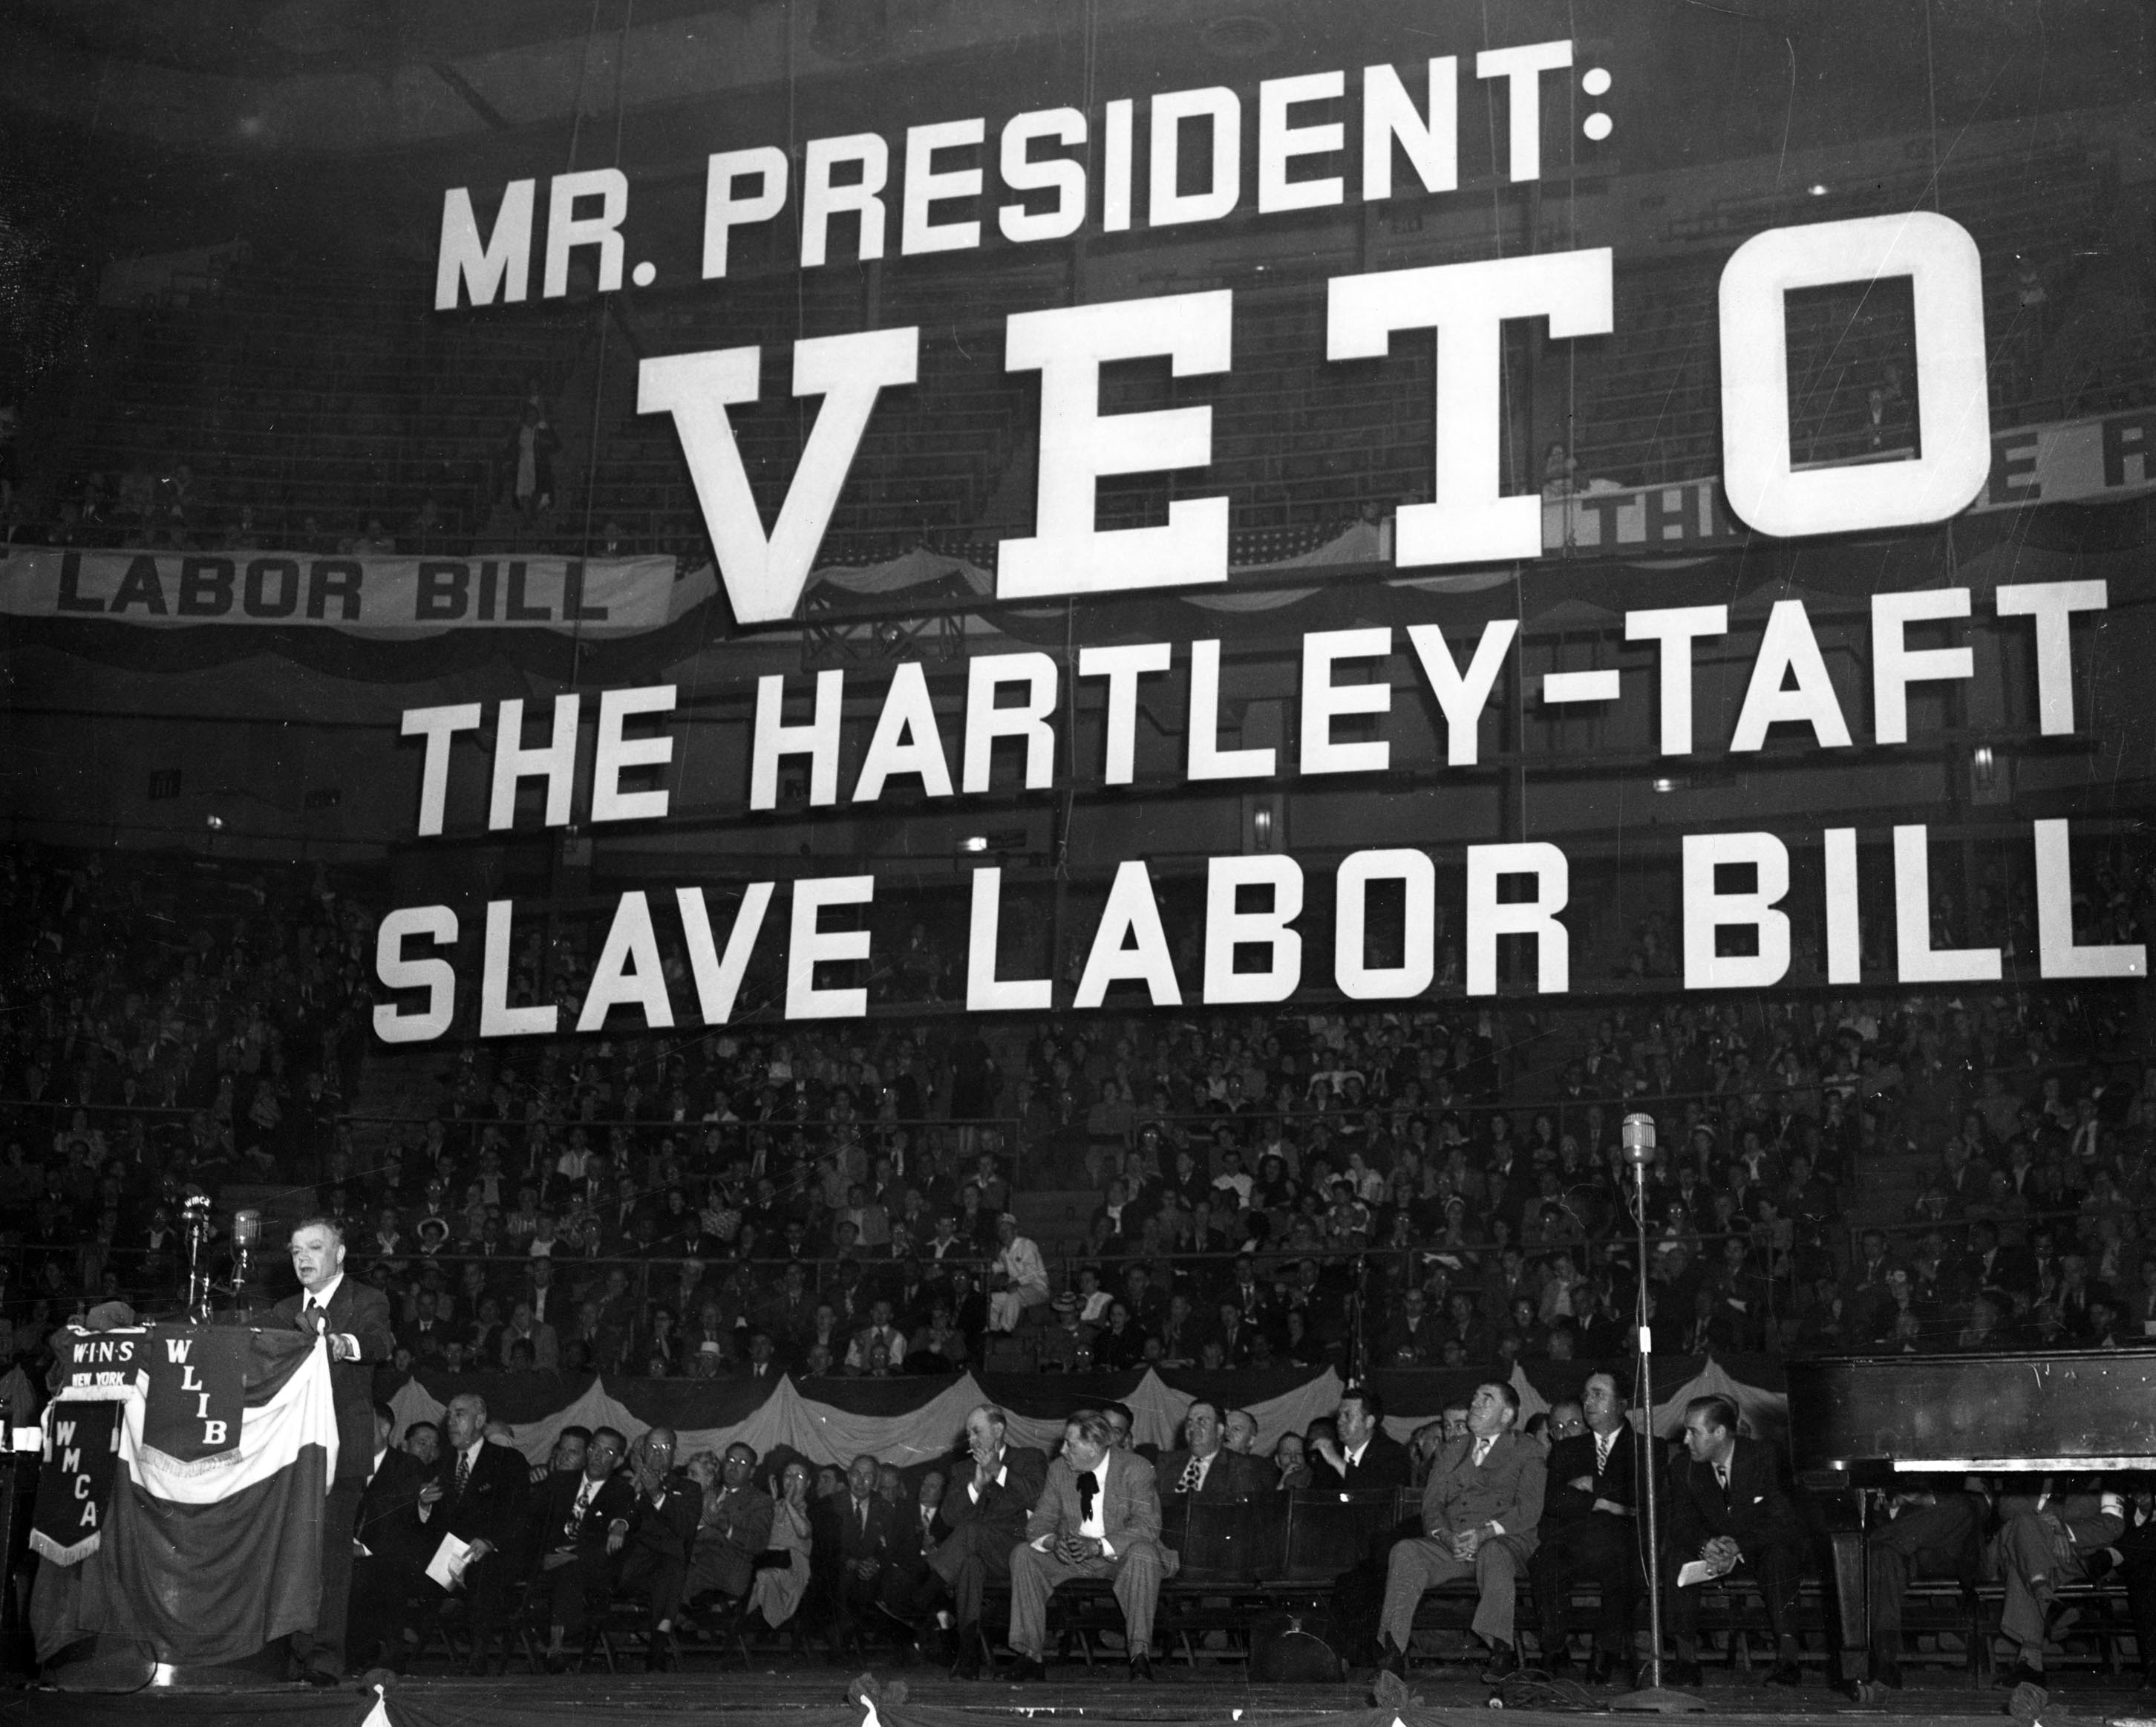
\includegraphics[width=\imageWidth]{images/slave_labor_bill}
  \captionsetup{justification=centering, singlelinecheck=false, margin=2cm} 
  \caption[Anti-Hartley-Taft Rally]{David Dubinsky of the \acrfull{ilgwu} gives a speech against the Hartley-Taft bill, with Luigi Antonini in the audience, May 4, 1947.\\ (Source: \href{https://www.investopedia.com/thmb/VcswppMRTl8IqMbgLRqdigfIGvs=/1500x0/filters:no_upscale():max_bytes(150000):strip_icc()/5278798677_0429e6aa05_k-7b6b81bdbbe44cdb929c08c7da9f8d29.jpg}{Investopedia.com}) \nocite{investopediaMrPresidentVeto}}
  \label{fig:slave_labor_bill}
\end{figure}

These years preceded the formation of the Oil Chemical and Atomic Workers (\acrshort{ocaw}). It wouldn’t be until March 4, 1955, when the \acrfull{ugccwa} merged with the \acrfull{owiu} to form the \acrshort{ocaw} (\cite[48]{ocawFactBookOil1960}). This was also the year when the \acrshort{afl} and \acrshort{cio} also merged, forming the present-day \acrfull{aflcio}.

\subsubsection*{The Oil Workers International Union}

Oil workers’ first breakthrough in terms of organizing occurred during World War I in Texas and California. The \acrfull{cio} had not yet formed, so a charter in the \acrfull{afl} was granted to several local unions; once several of these locals were chartered, they successfully petitioned the \acrshort{afl} for a charter as the Oil Field, Gas Well and Refinery Workers of America in 1918 (\cite[48]{ocawFactBookOil1960}). After some initial success, the union’s membership began to decline to merely 350 by 1933 because of union busting aided by the federal government, but the passage of the \acrfull{nlra} in 1935 gave the union a new set of rights and tools to organize, which again gave the union a boost (\cite[49]{ocawFactBookOil1960}). That same year, the president of the union worked with other labor leaders to establish the Committee for Industrial Organizations, though they remained within the \acrshort{afl}; but this did not last long, and two years later the Committee broke with the \acrshort{afl} to form its own union federation (\cite[49]{ocawFactBookOil1960}). During the same period, the union’s internal democracy considerably improved with the creation of the rank-and-file International Executive Council, and the convention no longer elected officers; instead, they were elected by direct referendum (\cite[49--50]{ocawFactBookOil1960}).

\subsubsection*{Gas, Coke, and Chemical Workers}

The Gas, Coke, and Chemical Workers Union started in the \acrfull{umwa}. The \acrshort{umwa} wanted to unite workers in industries that processed or used petroleum coke in the production of artificial gas (\cite[50]{ocawFactBookOil1960}). The \acrshort{umwa} was in the \acrshort{afl} at the time, and the Federation was resistant to their organizing efforts. After the \acrshort{umwa} left the \acrshort{afl}, it formed District 50, which was focused on organizing the "gas, coke, and allied products" industries (\cite[50--51]{ocawFactBookOil1960}). However, soon John L. Lewis, who was president of the \acrshort{umwa} at the time, split with the \acrshort{cio}, pulling the Mine Workers out of the \acrshort{cio}. This did not sit well with the Gas-Coke Workers within District 50; they had developed loyalty to the \acrshort{cio}, and were now merely a division within the now independent District 50 (\cite[51]{ocawFactBookOil1960}). Because of this, the various local unions of Gas and Coke Workers sought their own national union, and in 1942, they were granted a charter from the \acrshort{cio} as the United Gas, Coke and Chemical Workers of America (\cite[51]{ocawFactBookOil1960}). No longer a part of the independent District 50, they were now back in the \acrshort{cio}. But by 1955, they decided to merge with the Oil Workers to form the \acrfull{ocaw}.

In the years before Tony Mazzochi entered the union, anti-communism was in full force. The Gas-Coke \acrshort{ugccwa} local union Mazzocchi had joined had a close affiliation with the Communist Party. Several prominent leftist union leaders, such as Fred Hamilton and Charles Doyle, were key to the union’s strength and survival. Not only had several leftist leaders organized the Rubinstein plant that Mazzocchi worked in, but the founding convention of United Gas and Coke Workers \acrshort{ugccwa} was held near Doyle’s home area of Niagra Falls (\cite[81]{leopoldManWhoHated2007}). Unlike many of the craft unions of the time, which were practically all white and male, Gas-Coke \acrshort{ugccwa} was forthright in its opposition to discrimination. They were early adopters of anti-racist policies and practices. They passed resolutions condemning racist discrimination at their founding convention and urged for the promotion of more women in union leadership. Suffice it to say that despite the reactionary tide, the union managed to forge a genuinely progressive agenda, especially in light of the context in which they were operating.

Anti-communism, by and large, had not infiltrated the union’s rank and file either. For example, in 1946, the union voted to "provide financial support for the CP-dominated United Electrical Workers during its difficult Phelps-Dodge strike" (\cite[84]{leopoldManWhoHated2007}). Notwithstanding the strong CP presence within the union, it still counted many anti-communists amongst its ranks, though they managed to work together relatively peacefully until 1946 (\cite[84]{leopoldManWhoHated2007}). It was at that time the anti-communists began plotting to take over the union and push the communists out. They eventually purged Charles Doyle from the union by holding a convention in Canada. Doyle did not have legal immigration status in the US. The anti-communists tipped off the INS so that when Doyle tried to reenter the US, he would be denied. This effectively ended his \acrshort{ocaw} tenure. Jack Curran, an anti-communist, rose to power within the \acrshort{ocaw}.

Mazzocchi had connections with the CP through family and relatives, though Mazzocchi himself was not a member of the party. He was, however, politically active and looking for a job. At the same time, the purged communists were looking for revenge and to take back the union from Curran and the anti-communists. Mazzocchi got his start in the union as part of this effort. In moderating the politics of the union, Curran had been ineffective at warding off the "power grabs" by management. Furthermore, the chief steward had let grievances pile up unaddressed (\cite[90]{leopoldManWhoHated2007}). This presented an opportunity for Mazzocchi to step in and slowly organize to win workers over to his vision of what the union ought to be. He started by agitating around the inadequate handling of grievances at the Rubinstein plant where he worked and eventually ousted the conservative steward at the plant. Slowly, he worked through the ranks of union leadership, getting elected to the local committee at the Gas-Coke District Council and speaking up about issues at union meetings (\cite[97--98]{leopoldManWhoHated2007}). 

Over the years, the union maintained itself as a progressive voice within the labor movement. Despite having so many members in industries that work with environmentally hazardous chemicals, the union developed a plan for what it called a Just Transition: an effort to advance a politics that both protected the environment from hazardous chemicals and emissions and the workers who would be affected the most by transitions away from those processes and usage of those chemicals. Indeed, in the 1990s, the union spearheaded the effort to build the US Labor Party, a party independent of the Democrats and Republicans anchored in the trade unions. It also was instrumental in the creation of the \acrfull{csb} after the explosion at the Phillips Chemical Plant in Pasadena, Texas killed 23 workers.\footnote{Author correspondence with Mark Dudzic (\citeyear{dudzicInterview2024}).} The \acrshort{ocaw} was heavily supported and pushed for the passage of the Occupational Safety and Health Act, which created a federal agency to enforce occupational safety laws. The union was also a driving force in the passage of the Environmental Protection Agency (\cite{leopoldManWhoHated2007}).

Though the union maintained a progressive voice within the labor movement throughout the period, it continued to shed members throughout the 1980s and 1990s, largely to offshoring of production, automation, and deindustrialization. For example, plants that used to require 10,000 workers to operate now can be run with as few as 600 or 700 (\cite{dudzicInterview2024}). Ironically, many of the stringent occupational and environmental health and safety laws that the union advocated for also made production more expensive in the US and possibly contributed to the union’s decline in membership via offshoring and globalization. According to Mark Dudzic, a former \acrshort{ocaw} official, one employer was quite open about what drove their decision to move production outside the US. Over the years, the union had fought to improve safety at one of the plants where they had members. Approximately 120 workers at the plant were frequently exposed to very hazardous chemicals; the union finally convinced the employer to build a wastewater treatment plant and install enclosed production booths to mitigate the hazards. However, the company eventually decided to move production to India because of the costs. The union tried to negotiate with them to no avail. The company had a  \textdollar 10 million annual wage bill and environmental compliance costs of  \textdollar 15 million per year. In India, environmental compliance costs were close to zero and wages much lower (\cite{dudzicInterview2024}). According to Dudzic, the company told the union:

\begin{quote}
Our wage bill is \textdollar 10 million a year. Our environmental compliance is \textdollar 15 million a year. It's close to zero in India. So you could offer to work for free, and it still wouldn't be competitive with what we can do in India because of the environmental compliance. So, basically, they were offshoring not only our work but their ability to contaminate workers and communities. This plant had one of the highest rates of bladder cancer in the United States before we started organizing these protections, and I'm sure the rates of bladder cancer wherever they moved to in India went up because of this company. (\citeyear{dudzicInterview2024})
\end{quote}

In 1999, to "stop the bleeding," the \acrshort{ocaw} merged with the \acrlong{pace} (\acrshort{pace}; Figure \ref{fig:ocaw}). Dudzic described this merger as disastrous:

\begin{quote}
The [Paper Workers (\acrshort{upiu}) had] the opposite tradition in terms of internal governance. It was very top down, very closed; officers basically ran the show. They had these district directors who manipulated politics in the various districts, so it was very opposite of the \acrshort{ocaw}. Some people in our Union felt that we could shake things up; they promised to allow for some more democratic structures in the new Union, but they quickly closed the doors on that after the merger. The hope was that the paper workers were\ldots{}the structures of the industries were very similar, these large manufacturing facilities dominated by multinational corporations; the Paper Workers, like the Oil and Chemical workers \acrshort{ocaw}, had a lot of people in the South and rural areas. There was some sense that there could be some synergy there, but the leadership was backward, incompetent, and intent from the very beginning on purging any kind of militancy and progressive politics from the Union. (\citeyear{dudzicInterview2024})
\end{quote}

\noindent{}The merger also threatened the Just Transition framework that the \acrshort{ocaw} had pioneered:

\begin{quote}
[The \acrshort{upiu}] didn't like it [Just Transition]. We had this big fight about chlorine, which is a key ingredient in the paper-making process, but there [are] other technological ways to make paper without using chlorine. And we, the Oil, Chemical Atomic Workers (\acrshort{ocaw}), had called for a ban on chlorine. And the Paper Workers sided with the industry and opposed that ban; that was one of the first fights we had after the merger, and we lost, and that was sort of the defeat of the worker-centered, just transition model as opposed to an industry-supportive, "keep pumping the poisons out as long as you can" model. (\citeyear{dudzicInterview2024})
\end{quote}

\begin{figure}[!ht]
  \centering
  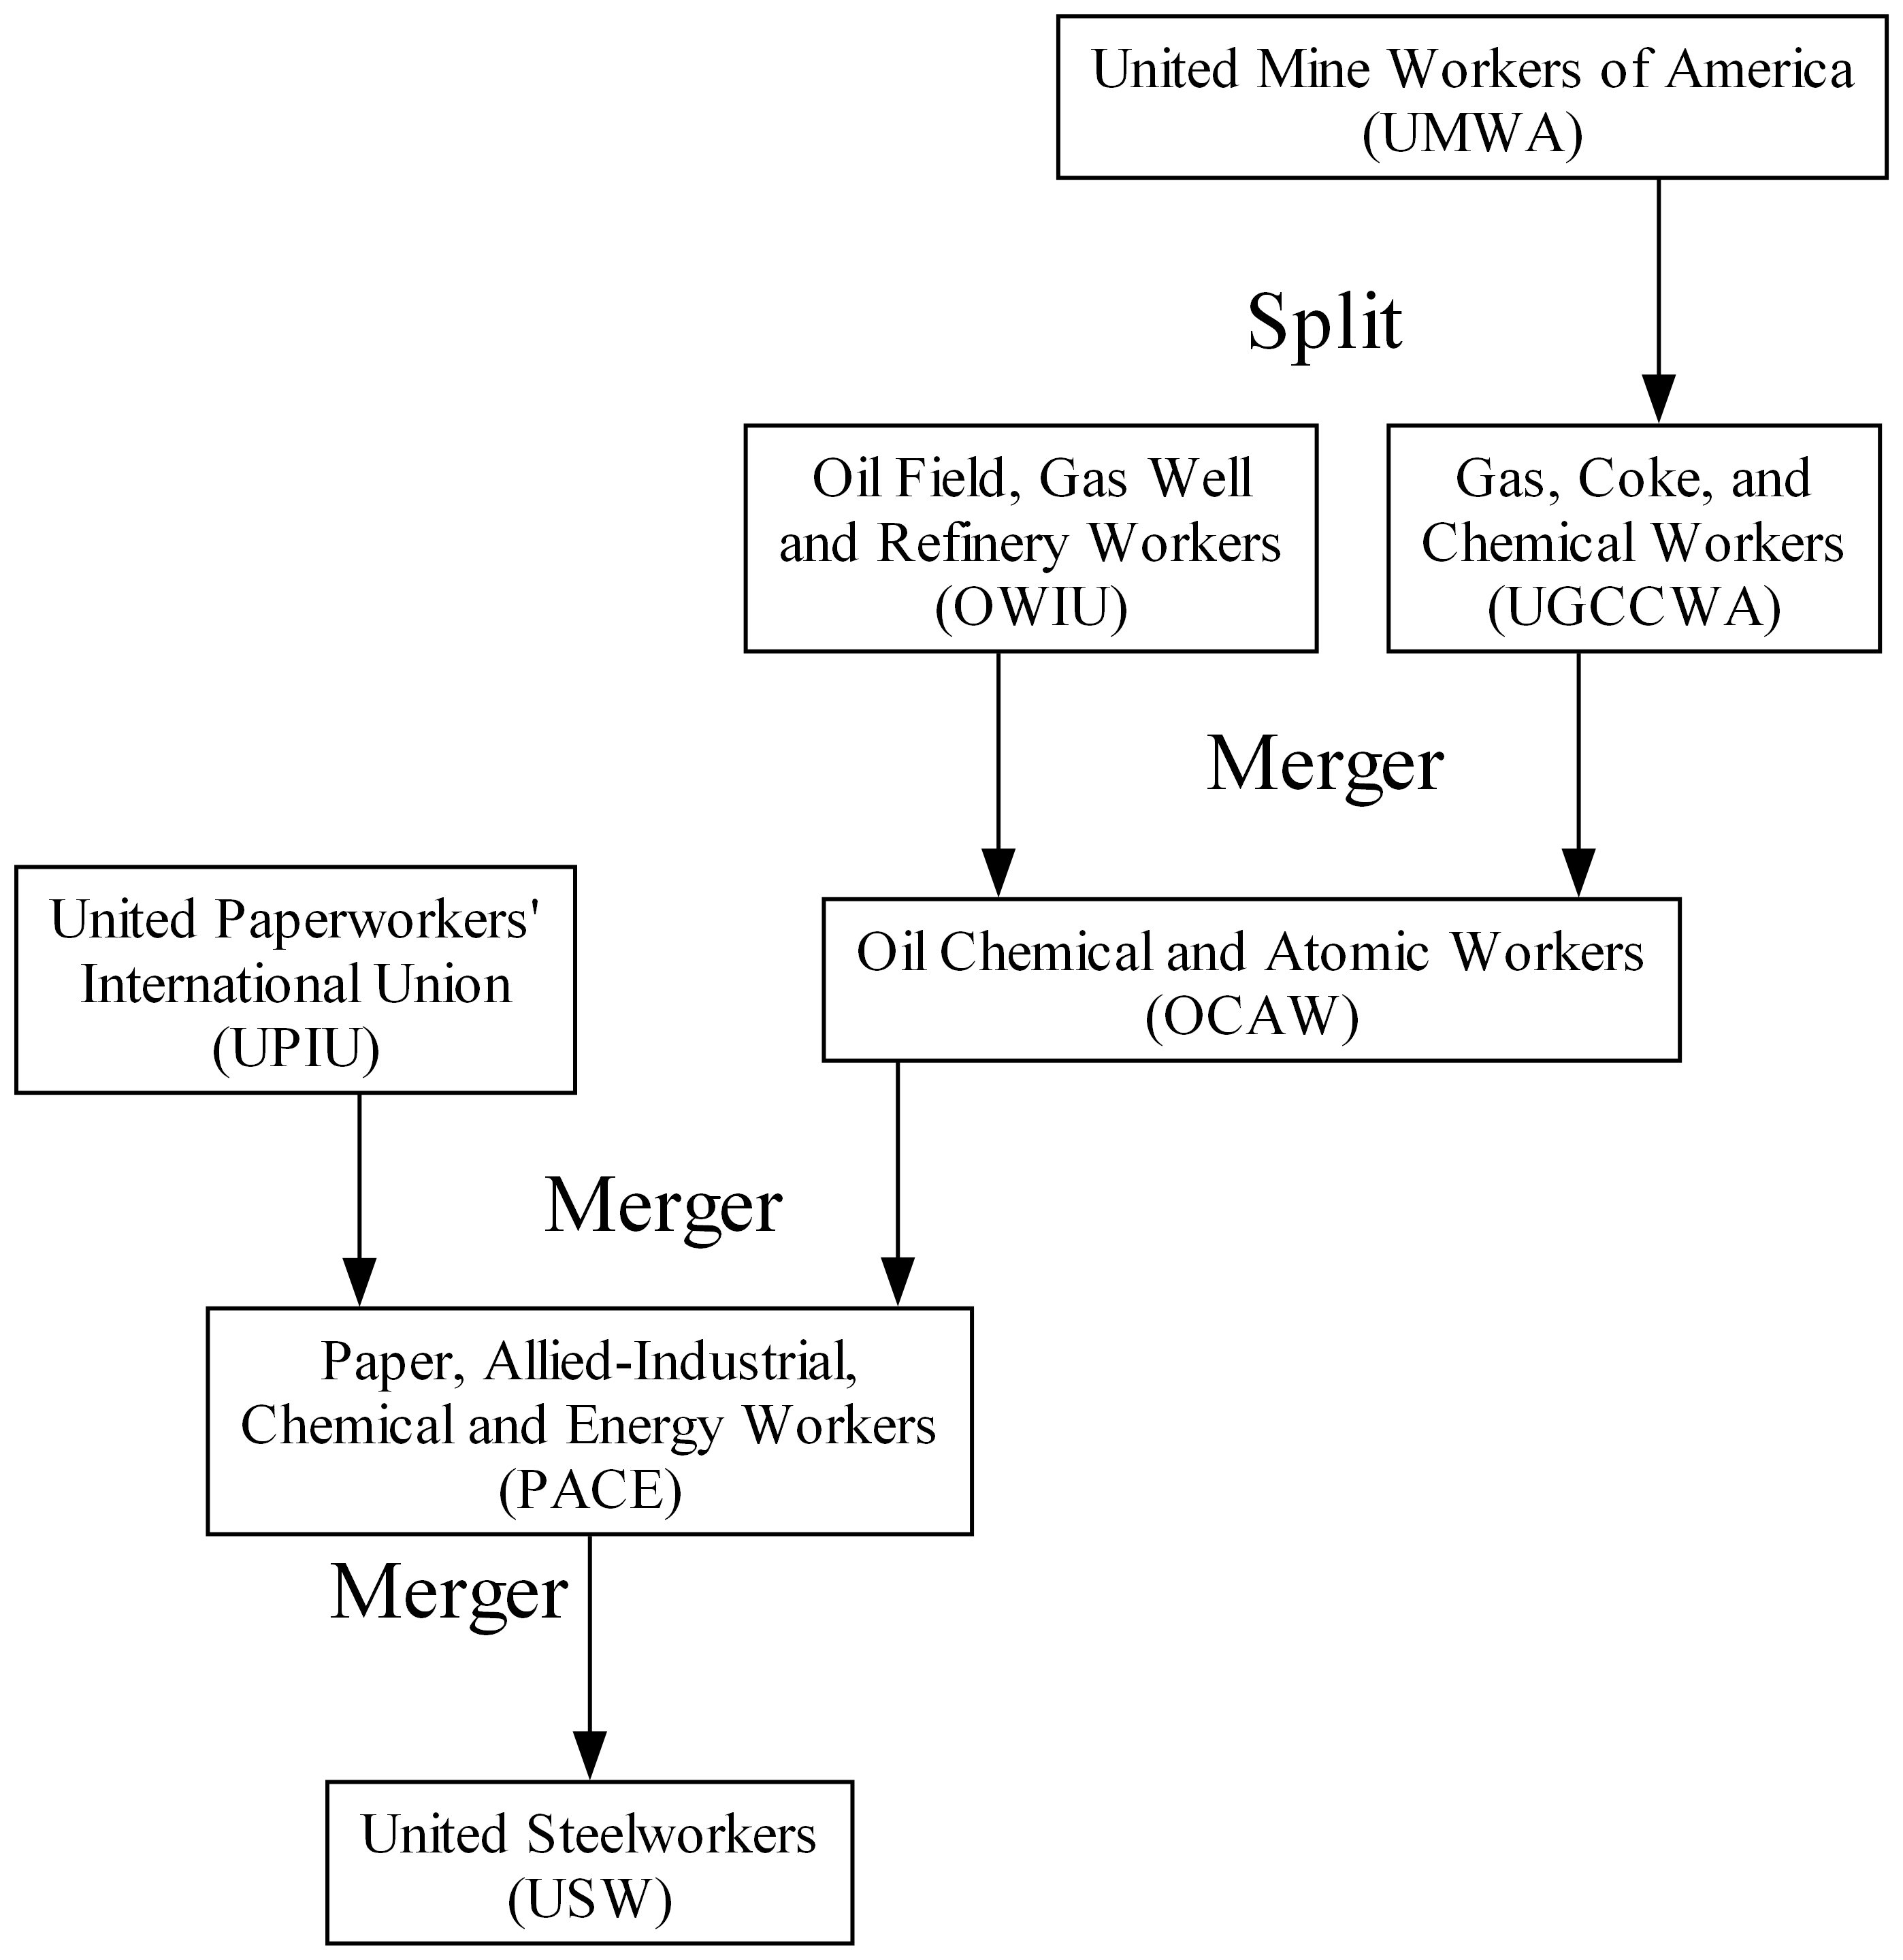
\includegraphics[width=\imageWidth]{images/ocaw}
  \captionsetup{justification=centering, singlelinecheck=false, margin=2cm} 
  \caption[Oil Chemical and Atomic Workers Mergers]{\acrfull{ocaw} was the product of a merger between the \acrshort{owiu} and \acrfull{ugccwa}. It merged with the \acrfull{upiu} in 1999 to form \acrshort{pace}. The \acrshort{ocaw} is now part of the United Steelworkers (\acrshort{usw})}
  \label{fig:ocaw}
\end{figure}

However, the merger was short-lived. In 2005, \acrshort{pace} was absorbed into the \acrfull{usw}. Though the merger with the \acrshort{usw} was also conducted in a top-down fashion (\cite{dudzicInterview2024}), it had the effect of stabilizing the union, which had remained in a precarious position after the previous merger. The two mergers have effectively wiped out many of the earlier \acrshort{ocaw} democratic rank-and-file decision-making processes and replaced them with more bureaucratic methods. For example, much of the negotiating activity is now carried out by "technicians," who closely study the economic trends in lieu of talking directly with the workers and "work[ing] from the bottom-up on\ldots{}bargaining" (\cite{dudzicInterview2024}). At the same time, the \acrshort{ocaw} culture around health and safety has survived. According to Dudzic, the \acrshort{usw} had "always [been] a partner with the \acrshort{ocaw}, from the days going back to the passage of the OSH Act in 1970" (\cite{dudzicInterview2024}). The \acrshort{usw}’s Health and Safety Department is also named after Tony Mazzocchi. It is called the Tony Mazzocchi Center for Labor and Environmental Health.

This persists even in 2023. To wit, the Carson, California \acrshort{usw} Local 675 has been supportive of several environmental initiatives and efforts. The Local, which it is important to note is an oil local, commissioned the Pollin Report released in 2021 (\cite{pollinProgramEconomicRecovery2021}). The report charts a path away from dirty fuel sources to clean energy. More recently, in 2023, Norman Rogers, vice president of \acrshort{usw} Local 675, was quoted in the \textit{Los Angeles Times} as a supporter of a transition from fossil fuel to clean energy jobs (\cite{rothCanClimateActivists2023}). Several local unions in the area have launched a political coalition to lobby Sacramento to protect workers while the transition occurs. From that perspective, perhaps the most enduring feature that has survived from the \acrshort{ocaw} days is the Just Transition framework.

\subsubsection*{Comparison: UA and the OCAW/USW}\label{compare_ocaw}

The \acrfull{ua} and \acrshort{ocaw}/\acrshort{usw} clearly organize very differently. The \acrshort{ua} along with \acrfull{nabtu} have been quite industry-friendly and reluctant to challenge the bosses because they rely on labor-management peace to maintain the relationship and keep the voluntary contract in place. This comes down to a highly pragmatic calculation about what the union perceives as areas where it has the upper hand because of skill level or other considerations, such as the employer's need for a large workforce that can quickly be deployed. Though the work can be skilled, as is the case with petrochemical work, the approach can still become conservative even in relation to those employers because of the ever-decreasing scope of \emph{highly skilled} work in general. That is, construction union leaders and members have taken a rearguard approach in the context of a limited pool of opportunities. Take the push for "clean energy" as an example. The Building Trades has been less than supportive of ending fossil fuel consumption and replacing it with renewables. Renewable energy companies have been notoriously anti-union, and unions have had little success in organizing workers in those companies (\cite{scheiberBuildingSolarFarms2021}). The unions see little else in the way of energy work and, thus, are not likely to challenge the industry.

The \acrshort{ocaw} is less burdened by the need to maintain friendly labor-management relations because they do not depend on voluntary contracts. Since labor-management peace is not necessary to keep the relationship in place, the  \acrshort{ocaw} challenges management more frequently and is more willing (and able) to take risks and align politically with other unions and progressive movements.

\subsection{The International Association of Machinists (IAM)}\label{iam}

The \acrfull{iam} and \acrshort{ua} are both craft unions. Both were \acrfull{afl} unions before the \acrshort{afl} and \acrshort{cio} merged in 1955. Although perhaps not anchored as steadfastly to the expansion of social-wage policy and decommodified public goods as unions such as the National Nurses United and National Health Care Workers or even The Brotherhood of Maintenance of Way Employees, they have nonetheless given their official support toward the effort to establish single-payer healthcare in the United States, a policy that would eliminate private insurers and establish government-funded healthcare insurance that would cover all regardless of one's income or finances. This arguably is along the more "radical" edge of the US trade union movement, such as it is. What could explain this different outcome? Both the \acrshort{iam} and the building trades unions were early \acrshort{afl} craft unions. They both have a history of racist, exclusionary policies. A key difference, however, is that the \acrshort{iam} is not a construction union and thus cannot enter into voluntary "prehire" agreements; they cannot "organize the bosses."

\subsubsection*{The formation of the IAM}

Nineteen machinists created the \acrshort{iam} on May 5, 1888 in Atlanta, Georgia \parencite{iamawHistoryIAMTimeline}. Unlike the industrial unions, the \acrshort{iam}'s history traces back not to mass production factory work but to the early fraternal labor association called the Knights of Labor. Unlike the militant \acrfull{cio} of the 1930s, the Knights of Labor emphasized individual moral improvement and had "some of the trappings and traditions of a secret society or fraternal order" \parencite[3]{perlmanMachinistsNewStudy1961}. This Knights of Labor influence melded with the nonegalitarian "Southern influence" that promoted the "superiority" of white, highly skilled labor \parencite[3]{perlmanMachinistsNewStudy1961}. This influence, in contrast to the Knights of Labor, which accepted anyone "who `lived by the sweat of the brow,'" was highly moralistic \parencite[5]{perlmanMachinistsNewStudy1961}. The last influence, which eventually became fully dominant, was that of a "pure and simple" unionism: the "concentration on the problems of effective job control" and an "emphasis on the mutuality of economic interest of all machinists regardless of their personal attitudes toward morals, mores, or men, in contrast with the Southern influence" \parencite[4]{perlmanMachinistsNewStudy1961}. This last influence put the union squarely in line with other craft unions of the Samuel Gompers \acrshort{afl} era.

In the earliest years, the union was highly moralistic. Its early governing documents limited membership to those machinists who were morally upright and explicitly sought to keep out "lesser men" whose immorality could compromise the newly formed Order.\footnote{At the time, the union was also referred to as the "Order of United Machinists and Mechanical Engineers of America," indicating the fraternal order character of the organization \parencite[5]{perlmanMachinistsNewStudy1961}.} The organization sought to bring together "machinists of ‘honorable, industrious and sober habits,’ who were being adversely affected by that ever-present minority, ‘which has destroyed the good reputation of the majority’" \parencite[5]{perlmanMachinistsNewStudy1961}. In its 1888 circular, Thomas W. Talbot, one of the Order's founding members, issued a statement that, unlike those "labor agitators," he believed that "the only right way of obtaining greater consideration is by persistently showing that we are more worthy men and better mechanics than formerly, thereby proving to our employers and the world at large that we are justly entitled to standing and distinction," and that this could only happen by the organization distinguishing itself "from lesser men, that is, those without equal social standing and equal craft skill"; another circular specified that membership was only offered to white, free born citizens who were paid "the average rate of wages given in some regulated machine shop and [the] trade," \parencite[5--6]{perlmanMachinistsNewStudy1961}. The latter restriction was aimed at filtering out those who were not the "highest skilled." This was the high point of the "Southern influence."

But as the union grew and expanded into the North, the color line in particular came under attack. Machinists in the North did not acknowledge the color line and the machinists union in New York City even refused to affiliate with the national machinists union until the color bar was removed from the union's constitution \parencite[9--10]{perlmanMachinistsNewStudy1961}. Dropping the color bar continued to become more important as the union sought additional allies in the labor movement. The machinists union could not win strikes alone, so it sought to affiliate with Samuel Gomper's \acrshort{afl}. However, Gompers refused to allow unions with "whites only" clauses to affiliate; despite both the \acrshort{iam} president and Gomper's urging of the convention delegates to vote to drop the "whites only" qualification so that the \acrshort{iam} could affiliate with the \acrshort{afl}, the delegates ultimately refused \parencite[16]{perlmanMachinistsNewStudy1961}. 

{\color{red}[Add more...]}

\subsubsection*{District Lodge 751}

Boeing workers in Washington's Puget Sound area formed \acrshort{iam} District Lodge 751 in 1935. This places the formation of the union directly in the context of the years in which the fledgling \acrshort{cio} was organizing workers in the rapidly expanding industries of the time. The \acrshort{cio}'s organizing tactics were influenced by the \acrfull{iww}, a radical union that pushed for the replacement of wage labor and the private ownership of industry with industrial democracy, where workers would collectively own the means of production and collectively make decisions about how the workplace should be run (\cite{industrialworkersoftheworldIWW}). Though the \acrshort{iww} remained politically marginal, their tactics and philosophy undoubtedly had an impact on the \acrshort{cio} in the 1920s and 1930s (\cite[2-6]{mccannBloodWaterHistory1989}). The \acrshort{afl}, committed to craft unionism, was unable to organize the new industrial workers because of disputes that would arise regarding which craft union the newly organized industrial workers should join. When the AFL did organize industrial workers, they would first organize them into industrial-like union structures called "federal" unions. Eventually, these unions were supposed to dissolve, with the workers reassigned to the appropriate craft union. However, many of the newly organized industrial workers were not attracted to the craft union idea, as evidenced by their continuing attendance at the "Federal" (i.e., industrial) union that they were initially organized into and their failure to attend the union meeting for their particular craft (\cite[8]{mccannBloodWaterHistory1989}).

In the 1930s, when the Boeing shop first unionized, the \acrshort{cio} was primarily focused on the auto industry. The workers experienced terrible conditions at work, and there had been talk about forming a union. Boeing had considered forming a company union, a union that is controlled by the employer and is not a truly independent labor organization, which was a popular tactic for many companies at the time. But with the passage of the \acrshort{nlra}, company unions became illegal, and Boeing recognized that, despite the pending legal challenges against the \acrshort{nlra}, the prospect of successfully forming a company union seemed unlikely; indeed, shortly after the company announced its intent to create a company union, the District Lodge filed a \acrshort{nlrb} complaint, and Boeing retracted its plan (\cite[23-24]{mccannBloodWaterHistory1989}). Furthermore, the \acrshort{cio} was on the rise and mounting militant challenges to employers in the auto industry, and Boeing thought that it would only be a matter of time before the growing labor federation turned its sights on Boeing. District Lodge 751, by contrast, was rather small, with only 35 members, and was not anchored in radical unionism \`{a} la the \acrshort{iww} or \acrshort{cio}. (\cite[24]{mccannBloodWaterHistory1989}). Within this context, it made quite a lot of sense for Boeing to choose what it saw as a lesser evil. So it chose to recognize District Lodge 751 as the workers' union.

The initial years of bargaining were generally amicable. Boeing agreed to all of 751's "non-cost" demands so long as 751 was willing to forgo any wage increases or other items that would directly increase Boeing's labor costs and alarm their creditors. But the friendly relations between District Lodge 751 and Boeing were short-lived. 

{\color{red}[Placeholder for discussion about more recent craft-unionism IAM vs ILWU fights.]}

\subsubsection*{Comparison between the Building Trades and the Machinists}

Notwithstanding the craft union orientation of the \acrfull{iam}, the union has taken the bold step of endorsing single-payer healthcare. They both have become an affiliate with the \acrfull{lcsp} and made an official commitment by passing a resolution at the union's 2004 convention \parencite{unionsforsinglepayerhealthcareUnionsSinglePayer, lcspLaborCampaignAffiliates}. No construction unions are affiliated\footnote{Affiliate is a higher standard than merely expressing support. It requires the union to pass an official resolution and a commitment to a single payer healthcare worker education program.} with the \acrshort{lcsp}, and none that this author is aware of have passed official resolutions expressing support for the same, though there have been sporadic expressions of support for single payer from the \acrlong{ibew}\footnote{Author correspondence with Mark Dudzic (\acrshort{lcsp}).} and the \acrlong{iupat} \parencite{unionsforsinglepayerhealthcareUnionsSinglePayer}.

% glsentrylong{ibew} 

\section{Comparisons between building trades unions}\label{intracases}

While the Building Trades largely "organizes the bosses"\footnote{A wonderfully apt description that I owe to Mark Dudzic, former \acrshort{ocaw} official and long-time \acrfull{lcsp} organizer.} rather than the workers already employed, there is still some variation in how they organize. Some construction unions file representation cases---meaning they follow the "industrial" organizing path rather than the construction path (Figure \ref{fig:organizing_paths}). Representation cases are filed when a group of workers or the union believes that a majority of the workers want the union to be officially recognized at their workplace. If successful, the employer has a legal obligation to negotiate with the union. These cases represent a departure from the usual approach that most building trades unions take. I expected construction unions that use the more typical organizing technique associated with the industrial unions in the 1930s\footnote{Many of the unions that use this method are not "industrial" in the way that the term was initially used in the 1920s and 1930s to denote manufacturing plant employment, such as automobile production lines, but the important point is that the "organize the workers" method that the \acrshort{nlrb} elections were established to accommodate is being used.} -- i.e., they organize workers in the workplace from the "bottom-up" -- would also take more progressive stances on other issues, be more likely to work with other unions on shared issues or concerns, and in general be less parochial and take a more expansive view of being pro-worker (e.g., endorse social wage policy such as single-payer healthcare that would benefit more than just their members.) The logic behind this expectation is that those construction unions who are using the "industrial" organizing technique are using inherently more confrontational or coercive tactics and thus could be more likely to see other progressive or left-wing organizations and unions as allies.

However, the interviews revealed that those construction unions who filed representation cases largely did \emph{not} embrace more progressive or left-wing politics. They usually used the technique for pragmatic reasons. For example, some workplaces were comprised of more permanent staff members who were not construction workers, and thus, the "industrial" technique was more appropriate anyway. By and large, these organizing undertakings did not lead the union to embrace more militant or progressive views.

\subsection{Millwrights}\label{millwrights}

A Millwrights local union in the Midwest organized workers at an agricultural plant after the workers reached out because they were not being treated with respect, were often asked to work outside of their classification without additional pay, and promises from management were continually broken. Since the workers were working permanently at a plant doing maintenance, they were technically not construction workers, and the union organized them the "industrial" way using an \acrshort{nlrb} election. The Millwrights Union was successful (they won the election). They organized alongside the International Brotherhood of Electrical Workers, who also successfully conducted an \acrshort{nlrb} election, and now both unions are trying to negotiate a contract with the employer.

The local union appeared to have limited involvement with other labor, community, or political organizations or campaigns. The organizer said that the local union did not have involvement in the local or county labor council,\footnote{It may be that the local union \emph{is} involved in the county labor council, but the organizer was unaware of the involvement. Most local unions at least have some affiliation with their regional or county-level labor council. Nevertheless, it seems safe to say that involvement in the county labor council is limited, at best.} but they were involved in the local building trades council, which is similar to the county labor federation but strictly for the building trades unions. In short, their inter-union collaboration seemed not to extend much beyond the building trades. Similarly, the local union largely took an apolitical perspective in terms of endorsements. The local union does not endorse any political candidates. Taken together, this suggests that there is not an association between more radical or progressive political activity and these organizing efforts. However, this also was the first organizing drive like this that the union had undertaken, and the organizer was quite excited about the possibility of more organizing drives like this one. So it remains to be seen what might happen to the union's political culture if they continue to take on organizing drives like these that respond directly to worker grievances.\footnote{It also could be that there is no relationship between these sorts organizing drives and the union's political culture, but the main point is that the local union could change politically as they undertake more "industrial-style" organizing.}

\subsection{Electricians (IBEW)}\label{ibew}

The \acrshort{ibew} local union experienced a similar situation when a group of upset workers reached out to the union for help. Workers at a telecommunications company were upset with the changes after the company was purchased and restructured. In particular, they were unhappy with the way that the company was treating them and the lack of respect from management. Because the local union also represents a number of utility and municipal workers in the city and, according to the organizer, had developed a reputation as a strong union, many union staff already knew the workers in the community. The union successfully won the \acrshort{nlrb} election, but in a tragic turn of events, the company decided to lay off all their installers and replace them with subcontractors. The union is now trying to negotiate a layoff package instead of a first contract.

That so many in the local community already knew the union and its importance to workers---i.e., it had built a good reputation---suggests that the union could be somewhat broader in its orientation (i.e., not narrowly focused on its members to the exclusion of broader issues). However, this seems not to be the case. The local union seems to be no different from the building trades unions in general in terms of their political culture. They still tend to take a rather careful approach of trying to win employers over versus more militant strategies (e.g., organizing for a strike), although they did indicate that they were involved in the county labor council and the building trades council (multi-union federations), which suggests that there is at least nominally some inter-union solidarity.
%It is encouraging to see that the union has established itself as an organization that workers can contact to help them organize and defend themselves. This is also important in terms of understanding how the union engages with the broader community.

\subsubsection*{Project labor agreements}\label{plas}

One area in which the \acrshort{ibew} local was quite politically active in the community is in urging local government to adopt project labor agreements. A \acrfull{pla} is a "\ldots{}pre-hire collective bargaining agreement with one or more labor organizations that establishes the terms and conditions of employment for a specific construction project\ldots{}" (\cite{obamaExecutiveOrder135022009}). The projects that a \acrshort{pla} covers are usually publically funded. Construction unions are attracted to \acrshort{pla}s because once they are enacted by the government (often at the local level), they are binding on all contractors who decide to bid on project for a particular institution (e.g., a school district) or a particular project (e.g., a new library; \cite{kotlerProjectLaborAgreements2009, johnston-doddsConstructingCaliforniaReview2001}). This forces employers who would otherwise not hire union workers to hire from the union's hiring hall and thus be bound by the union's contract for the duration of the project. With this technique, the union can capture part of the construction market that it otherwise would not be able to with the usual construction organizing method of "organizing the bosses."

%\begin{quote}
%[We] have had success [spreading awareness of] the benefits of community workforce agreements (\acrshort{cwa}s), which are similar to project labor agreements (\acrshort{pla}s) at the local level. 
%\end{quote}

At the same time, the adoption of these agreements is usually conditional on the incorporation of language promoting "labor peace." For example, the federal government requires \acrshort{pla}s to "contain guarantees against strikes, lockouts, and similar job disruptions." These conditions are often more restrictive and onerous than the no-strike clauses typically contained in most collective bargaining agreements (\acrshort{cba}s) with respect to what sorts of collective or concerted activity a union is forbidden from engaging in. Many \acrshort{cba}s contain a simple, straightforward "no strike/no lockout" clause that legally prevents both the union from striking and the employer from refusing to let the employees work for the duration of the contract.\footnote{Trade unionists with more radical leanings have critiqued the widespread acceptance of no-strike clauses within the labor movement, arguing that these clauses have significantly reduced labor militancy. See \citeauthor{burnsRevivingStrike2011} (\citeyear[Ch. 3]{burnsRevivingStrike2011}) for a detailed critique of no-strike clauses.} But \acrshort{pla}s typically contain language that, in addition to the standard no-strike language, also prohibits less aggressive tactics, such as hand-billing\footnote{Distributing fliers or leaflets advising the public of a labor dispute or political action.} or even "advising the public that a labor dispute exists" (\cite[7]{antiochunifiedschooldistrictProjectLaborAgreement2013}). For example, the Antioch Unified School District's \acrshort{pla}\footnote{I was unable to locate an agreement that the IBEW local in Alaska specifically has agreed to, but the others that I have found were consistently more stringent than collective bargaining agreements (CBAs). Moreover, parties to these agreements, especially the government, understand the centrality of "labor peace" to these agreements, so it is fair to make some generalizations based on the contracts that I did find.} for construction projects at Antioch High School requires that

\begin{quote}
There shall be no strikes, sympathy strikes, work stoppages, picketing, hand-billing or otherwise advising the public that a labor dispute exists, or slowdowns of any kind, for any reason, by the Unions or employees employed on any Project included within the scope of the applicable Projects, at the job site of any such Project or at any other facility of the District because of a dispute on a Project. Any such disputes are to be addressed through the dispute resolution process as set forth herein and in applicable law. (\cite[7]{antiochunifiedschooldistrictProjectLaborAgreement2013})
\end{quote}
By contrast, \acrshort{ua} Local 393's standard \acrshort{cba} is much less onerous and even allows for the union to observe sympathy strikes (refuse to work when other unions are on strike):

\begin{quote}
The parties hereto agree that while this Agreement is in effect, and while the other party hereto complies herewith, there shall be no strike, lockout or other work stoppage, except that it is understood that a stoppage of work because of any lawful primary picket line or one sanctioned by the Santa Clara-San Benito County Building Trades Council, shall not be a violation of this Agreement; and no employees shall be discharged, disciplined, suspended or laid off for honoring or refusing to work behind such picket line. (\cite[50]{ualocalunion393MasterLaborAgreement2018})
\end{quote}

From that perspective, \acrshort{pla}s have both class antagonist and class collaborationist elements. They are class antagonist in that they move the construction union away from the standard construction method of "organizing the bosses" to more coercive tactics. \acrshort{pla}s are inherently coercive in one sense because they force the employer to hire union regardless of whether the latter wants to. But they can often be class collaborationist\footnote{Although they are not \emph{inherently} class collaborationist in that the union and the government could agree to a project labor agreement that does not contain a no strike clause.} because of how closely the project labor agreement is tied to "labor peace."

In sum, the IBEW local's emphasis of \acrshort{pla}s does not represent much of a departure from what most building trades unions are doing. Pushing for \acrshort{pla}s is a common strategy that construction unions use in many parts of the United States. In that sense, it can \textit{not} be said that this local is more radical or class struggle oriented because of their emphasis of \acrshort{pla}s.

On the national level, the local supports some important legislative efforts and is vigilant when it comes to fighting right-to-work legislation. They also support the initiatives that the national labor federation (\acrshort{aflcio}) supports, including the \acrfull{proact}:

\begin{quote}
At the national level, there had been a pretty large effort to pass what's known as the \acrshort{proact} or the Protecting the Right to Organize Act, and that was at the national level. It hasn't been passed yet, but that was one in recent history.\ldots{}Of course, if there's ever an initiative to expand right-to-work legislation, we would certainly be opposed to that. I don't know that there has been a push either locally or nationally for that recently, but it’s always on our radar as well. (Interview with \acrshort{ibew} union organizer)
\end{quote}

\noindent{}However, this also does not represent much of a difference from what other building trades unions support. That notwithstanding, the \acrshort{ibew} local \emph{does} seem to be more politically active than the Millwrights local.

\subsection{Cement Masons and Plasterers (OPCIMA)}\label{opcima}

An \acrfull{opcima} local union organized excavation workers who had been working for a company that was not signed to a full agreement; the company was signed to a seasonal agreement. Because the agreement was seasonal, the workers were unsure if they would still have a job each spring. The workers were already union members, and they wanted the employer to sign a full agreement. However, the excavation company opposed the effort. Because of this, the union pursued an \acrshort{nlrb} election to force the employer to accept the union, \textit{fait accompli}. The union prevailed. The organizer explained that because most of these workers were already union members, this was an "easy case." The union mostly just had to maintain lines of communication to win the election. However, the union has still not reached a first contract; negotiations are ongoing. The union organizer suggested that, according to the union's lawyer, the company may already be bound to the union agreement because they have continued to employ the workers and pay into the union's Taft-Hartley trust fund.\footnote{Rather than the employer providing benefits, construction unions operate a trust fund to administer health and welfare benefits for their members.} Still, the case is ongoing and it remains to be seen what will happen.

The organizer has been involved with many similar organizing efforts that followed the "industrial" path. Many of them had been more contentious than this one. Yet, the union is still very cautious with how it handles workplace issues. For example, the way that the union handles workplace disputes is particularly cautious; the organizer explained that filing grievances was "bad business":

\begin{quote}
Every grievance or job site issue is handled completely differently [based on the context]. It really depends on the grievance or the issue. We, as a local, don't like grievances, and we don't like job site issues, and we don't like to file grievances ever. That's not our forte. It's kind of bad business. But at the same time, if push comes to shove and you have to file a grievance, usually, we do everything in our power to communicate. So, we're going to give the contractor the benefit of the doubt and do as much communication as we can.\ldots{}I'm currently in a grievance right now, but it's also [a situation where] the grievance itself isn't egregious. The grievance is just a placeholder to ensure that the member who's being aggrieved is protected. [It] gives us the opportunity to work with the contractor to hash out whatever issues or grievances are at hand. It gives us just legal teeth to\ldots{}hold them in compliance to protect our membership. (Interview with \acrshort{opcima} organizer)
\end{quote}

The political activity of the union was largely limited to community service-related work, though the organizer did indicate that the union also participates in local job fairs to recruit people into the trade:

\begin{quote}
[W]e're constantly doing outreach. We work with school districts and cities, and we work with the jail, the Department of Corrections. We work hand in hand with pretty much all the big players in the industry. We go to new job fairs and crap, or we'll do Habitat for Humanity and donate free labor. Or we collaborate on a macro level, whether it be organizing campaigns or communities in need; we'll do what we can to help out with financial needs, materials, or labor. We [also participate in] Toys for Tots.\ldots (Interview with \acrshort{opcima} organizer)
\end{quote}

Like the \acrshort{ibew} local, the more overtly political activity centered around advocating for local government to enact Project Labor Agreements (\acrshort{pla}s). The organizer emphasized that these agreements offer a pathway into well-paying, unionized construction jobs for many because in addition to requiring the employer to pay union wages and into union benefit trust funds, they also incentivize apprenticeship utilization, which creates more opportunity for members in the community. He also explained that the \acrshort{pla}s did not exclude any contractors from the bidding process and could actually be used to create new opportunities for minority contractors while ensuring quality control for the owner group. Through this process, the union can expose the non-union contractors to what the union has to offer and attempt to get the non-union contractors to become signatory.

As was the case with the \acrshort{ibew}, while the \acrshort{pla} process contains some coercive elements. It sought to force contractors paying below area standard wages to hire union workers, increasing workers' wages and benefits. This maintains a "floor" for wages and benefits, preventing non-union employers from placing low bids that union employers could not possibly compete with because of the higher wages and superior benefits package that they must pay into. However, it is also still heavily anchored in class collaboration and class peace. Although the union's \acrshort{pla}s can offer new opportunities to workers wanting to enter the construction industry, \acrshort{pla}s ultimately are being used by this local to persuade employers to join the union because of its benefits to employers as well. Significantly, this underscores the consequences of a voluntary contractual relationship on union strategy; even strategies that are at first blush coercive are ultimately integrated into a class conciliatory strategy.

\section{Conclusion}\label{conclusion}

{\color{red}[Conclusion goes here]}

% Uncomment to use end notes instead of footnotes.
%\theendnotes

%%%%%%%%%%%%%%%
%%%% Bibliography %%%%
%%%%%%%%%%%%%%%

% Start on new page
\clearpage
%\titleformat{\section}{\fontsize{12}{14}\bfseries\centering}{\thesection}{0.5em}{}
\titleformat{\section}[block]
	{\normalfont\fontsize{12}{14}\selectfont\bfseries\centering}
	{\thesection.}
	{0.5em}
	{\MakeUppercase}
	
% Line spacing
\setstretch{1.25}
\sloppy
\printbibliography[heading=bibintoc]% , title=REFERENCES]

\clearpage

% List of acronyms
\addcontentsline{toc}{section}{Acronyms}
%\setglossarystyle{listgroup}
\setlength\glsdescwidth{0.8\linewidth}
\printglossary[type=\acronymtype, title=Acronyms, style=long]
\clearpage

%\paperwidth=\pdfpagewidth
%\paperheight=6.5in
%\pdfpageheight=8.5in % keep at 8.5 in
%\pdfpagewidth=11in % keep this at 11 in
%\headwidth=8.5in % keep this at 11 in

%\fancypagestyle{lscape}{% 
%\fancyhf{} % clear all header and footer fields 
%\fancyhead[L]{%
%\begin{textblock}{1}(1,15){\rotatebox{90}{test}}\end{textblock}
%\begin{textblock}{1}(13,15){\rotatebox{90}{\thepage}}\end{textblock}
%}}

\begin{landscape}
%\pagestyle{lscape}
\clearpage

\paperwidth=\pdfpageheight
\paperheight=\pdfpagewidth
\pdfpageheight=\paperheight
\pdfpagewidth=\paperwidth
\headwidth=\textheight
\begingroup 
\vsize=\textwidth
\hsize=\textheight
\hfill
\begin{table}[!ht]
    \centering
    \fontsize{12}{20}\selectfont
    \begin{tabular}{@{}llll@{}}
        \toprule[0.25pt] \midrule[0.25pt]
        \textbf{Union} & \textbf{Similarity} & \textbf{Difference} & \textbf{Outcome} \\ 
        \midrule[0.25pt] \midrule[0.25pt]
        Machinists (IAM) & \multirow{2}{*}{\begin{tabular}[c]{@{}l@{}}Craft\\unions\end{tabular}} & \begin{tabular}[c]{@{}l@{}}• Industrial mode\\ \hspace{7pt} of organizing\\ • Involuntary agreements\end{tabular} & \begin{tabular}[c]{@{}l@{}}• Supports progressive social-wage policy\\ \hspace{7pt}(e.g., single-payer healthcare).\end{tabular} \\ 
        \cmidrule(r){1-1} \cmidrule(l){3-4} 
        Plumbers/Pipefitters (UA) & & • Voluntary agreements & • No/limited support for social-wage policy. \\
        \midrule[0.25pt] \bottomrule
    \end{tabular}
    \captionsetup{justification=centering, singlelinecheck=false, margin=2cm} 
    \caption[MSSD: IAM and UA]{The IAM and UA are similar in that they are both are craft unions, but only the UA is a construction union with voluntary agreements.}
    \label{tab:iam_similar}
\end{table}

\begin{table}[!ht]
    \centering
    \fontsize{12}{20}\selectfont
    \begin{tabular}{@{}llll@{}}
        \toprule[0.25pt] \midrule[0.25pt]
        \textbf{Union} & \textbf{Similarity} & \textbf{Difference} & \textbf{Outcome} \\ 
        \midrule[0.25pt] \midrule[0.25pt]
        \begin{tabular}[c]{@{}l@{}}Oil Chemical \& Atomic\\ Workers/Steelworkers\\ (OCAW/USW)\end{tabular} & \multirow{2}{*}{\begin{tabular}[c]{@{}l@{}}\\Petrochemical\\work\end{tabular}} & \begin{tabular}[c]{@{}l@{}}• Industrial mode\\ \hspace{7pt} of organizing\\ • Involuntary agreements\end{tabular} & \begin{tabular}[c]{@{}l@{}}• Supports progressive social-wage policy.\\• Supports the Pollan Report (creation of clean\\ \hspace{7pt}-energy jobs) and a transition from fossil fuels.\end{tabular} \\ 
        \cmidrule(r){1-1} \cmidrule(l){3-4} 
        Plumbers/Pipefitters (UA) & & • Voluntary Agreements & \begin{tabular}[c]{@{}l@{}}• No/limited support for social-wage policy.\\• Has defended the construction of\\ \hspace{7pt}new oil pipelines.\\• Opposed reforms and regulatory policies\\ \hspace{7pt} that might hamper new refinery projects\end{tabular} \\ 
        \midrule[0.25pt] \bottomrule
    \end{tabular}
    \captionsetup{justification=centering, singlelinecheck=false, margin=2cm} 
    \caption[MSSD: OCAW/USW and UA]{The OCAW/USW and UA are similar in that they both have petrochemical work, but only the UA is a construction union with voluntary agreements.}
    \label{tab:usw_similar}
\end{table}
\endgroup
\hfill
\clearpage
\begin{table}[!h]
\centering
\begin{tabular}{p{30mm}p{87mm}p{87mm}}
\toprule
\midrule
% Column Names
\begin{center} \textbf{Characteristic} \end{center} & % Col 1
\begin{center}\textbf{Non-construction Unions}\end{center} & % Col 2
\begin{center}\textbf{Construction Unions}\end{center} \\	% Col 3
\hline
\hline

% Row
\begin{center}\textbf{Initial Relationship}\end{center} &	% Col 1
\begin{center}\begin{flushleft}Involuntary: employers do not seek the union for workers\end{flushleft}\end{center} &	% Col 2
\begin{center}\begin{flushleft}Voluntary: employers seek the union for their “pool of skilled labor”\end{flushleft}\end{center} \\ % Col 3
\hline

% Row
\begin{center}\textbf{Employer Obligations}\end{center} & % Col 1
\begin{center}\begin{flushleft}Employer \underline{has an obligation} to continue bargaining after the contract expires\end{flushleft}\end{center} & % Col 2
\begin{center}\begin{flushleft}Employer \underline{has no obligation} to continue bargaining after the contract expires\end{flushleft}\end{center} \\	% Col 3
\midrule

% Row
\begin{center}\textbf{Employment Duration}\end{center} &	% Col 1
\begin{center}\begin{flushleft}Ongoing, long-term, or permanent\end{flushleft}\end{center} &	% Col 2
\begin{center}\begin{flushleft}Usually temporary; project-based\end{flushleft}\end{center} \\ % Col 3
\midrule

% Row
\begin{center} \textbf{Hiring} \end{center} &	% Col 1
\begin{center}\begin{flushleft} Hired directly by the employer \end{flushleft}\end{center} &	% Col 2
\begin{center}\begin{flushleft} Dispatched by the union to meet the employers' needs \end{flushleft}\end{center} \\ % Col 3
\midrule

% Row
\begin{center}\textbf{Organizing Method}\end{center} &	% Col 1
\begin{center}\begin{flushleft}Workers organize around their interests irrespective of the employer's desires \end{flushleft}\end{center} & % Col 2
\begin{center}\begin{flushleft}Union convinces employers of the union's benefit to them\end{flushleft}\end{center} \\	% Col 3
\midrule

% Row
\begin{center} \textbf{Majority Status\textsuperscript{\dag}} \end{center} &	% Col 1
\begin{center}\begin{flushleft} Required \end{flushleft}\end{center} &	% Col 2
\begin{center}\begin{flushleft} \underline{Not} Required \end{flushleft}\end{center} \\ % Col 3
\midrule
\bottomrule
%\begin{center} \textbf{Placeholder} \end{center} &	% Col 1
%\begin{center}\begin{flushleft} Placeholder \end{flushleft}\end{center} &	% Col 2
%\begin{center}\begin{flushleft} Placeholder \end{flushleft}\end{center} \\ % Col 3
%\midrule
\end{tabular}
	\captionsetup{justification=centering, singlelinecheck=false, margin=3cm} 
    \caption[Differences in Organizing and Contracts]{The charactersitics of each mode of organizing and contract type.}
    \label{tab:contracts}
\end{table}


\noindent\dag{} Whether the majority of the workers must want a union. This requirement makes it necessary to "organize the workers."

\end{landscape}

%\newpage
%\paperwidth=\pdfpageheight
%\paperheight=\pdfpagewidth
%\pdfpageheight=\paperheight
%\pdfpagewidth=\paperwidth
%\headwidth=\textwidth

\end{document}
